\documentclass[10pt,a4paper]{beamer}
\usepackage[latin1]{inputenc}
\usepackage[spanish]{babel}
\usepackage[T1]{fontenc}
\usepackage{amsmath}
\usepackage{amsfonts}
\usepackage{amssymb}
\usepackage{graphicx}
\usepackage{beamerthemesplit}
\usepackage{float}
\usepackage{multirow}
\usepackage{multicol}
\usepackage{url}
\usepackage{ragged2e}
\usepackage{array}
\usepackage{latexsym}
\usepackage{subfigure}
\usepackage{timing}
\usepackage{url}

\setbeamertemplate{footline}[frame number]
\setbeamertemplate{bibliography item}[text]
%\setbeamertemplate{subsubsection in sidebar shaded}
%{\tableofcontents[subsubsectionstyle=hide]}

%\usetheme{Montpellier}
\usetheme{Warsaw}
\decimalpoint
\renewcommand{\contentsname}{Contenido}

\begin{document}

\title{Integraci�n sem�ntica de \\ los recursos de informaci�n en \\ una memoria corporativa}
\author{Erik Alarc�n Zamora}
\date{Enero 2014. M�xico, D.F.}

\begin{frame}
\titlepage
\centering
Asesores:\\ Dra. Reyna Carolina Medina Ram�rez \\Dr. H�ctor P�rez Urbina
\\
\end{frame}
\begin{frame}
\frametitle{Contenido}
\setcounter{tocdepth}{1}  
\begin{scriptsize}\tableofcontents[]\end{scriptsize}
\end{frame}
\section{Contexto y motivaci�n}

\subsection{Memoria corporativa}
\begin{frame}
	\frametitle{Memoria Corporativa}
	%%%%%%%%%%%%%%%%%%%%%%%
	\begin{block}{Definici�n}
	\justifying 
	La representaci�n expl�cita, t�cita, consistente y persistente del conocimiento de una organizaci�n. \cite{Ontoinra2002}
	\end{block}
	
	\begin{figure}[htbp]
	\centering
	\subfigure{
	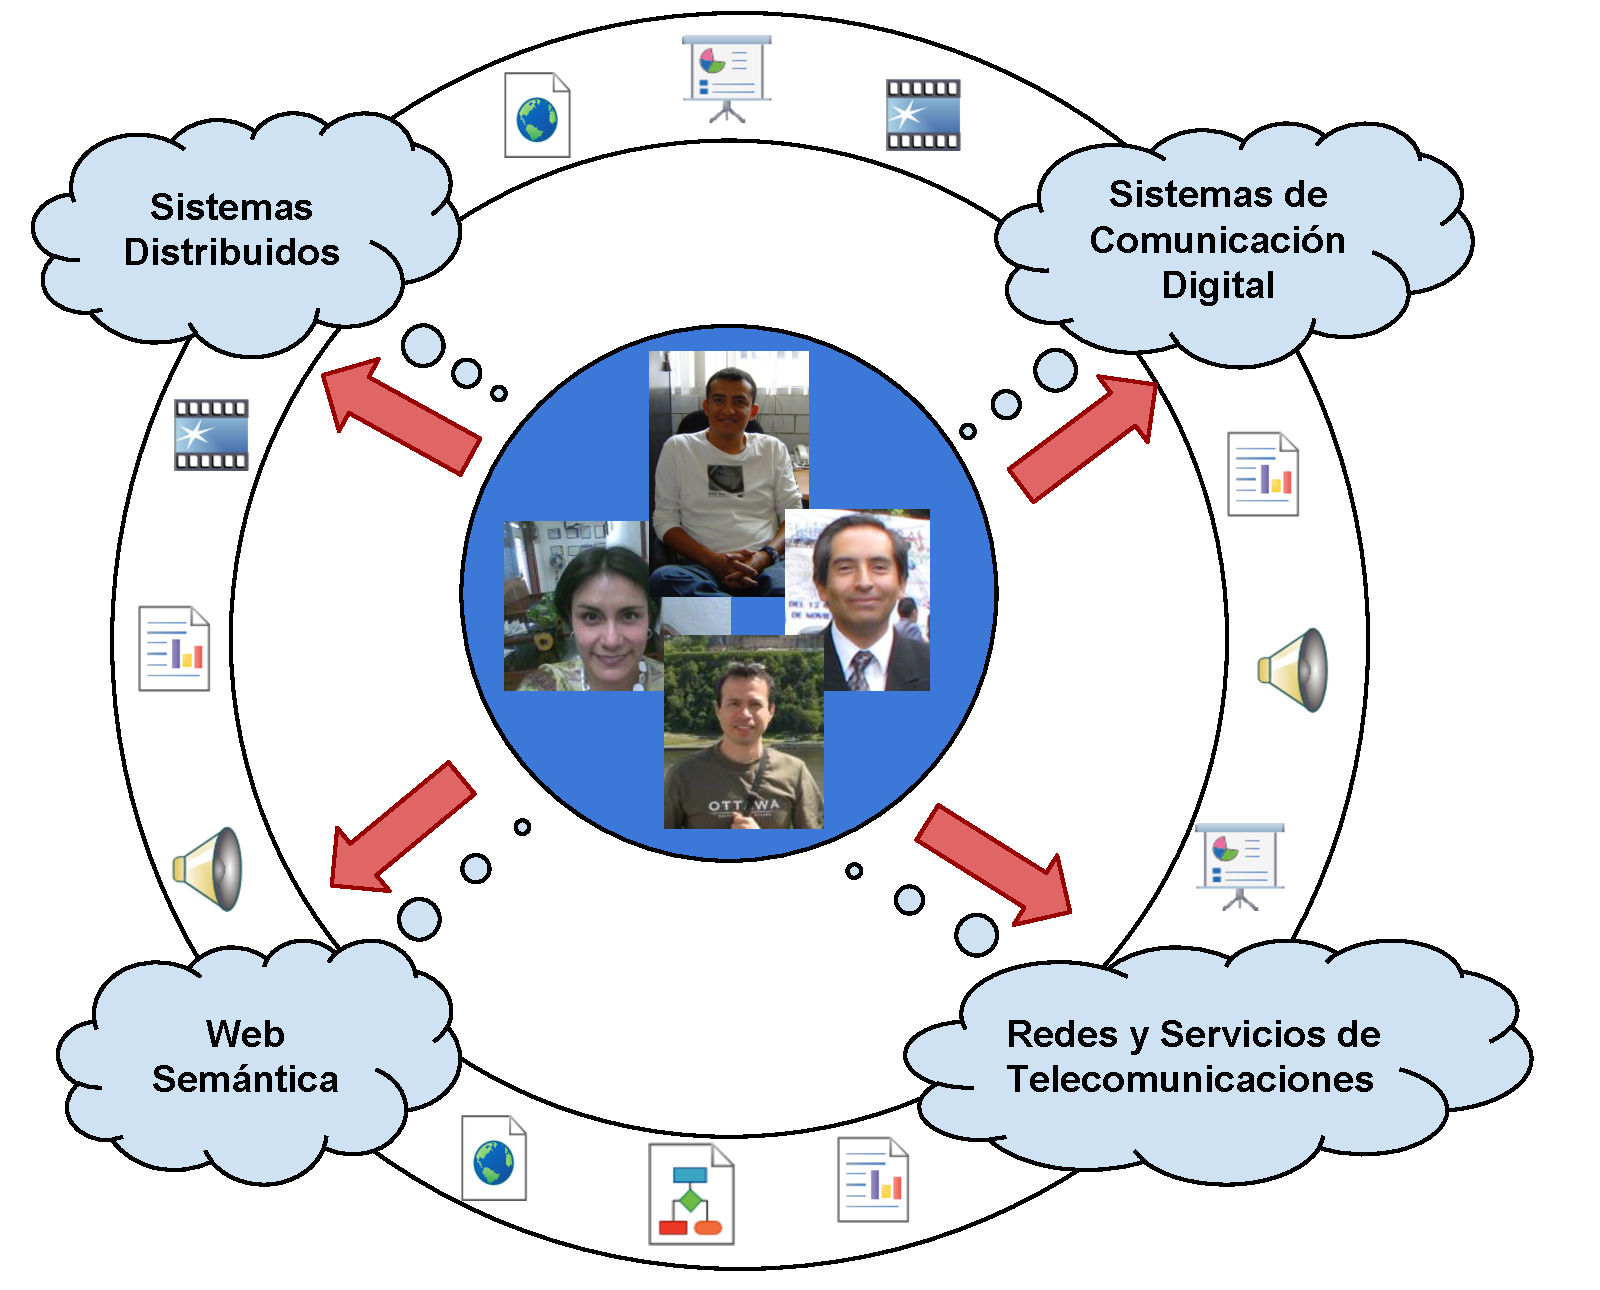
\includegraphics[scale=0.18]{ConocimientoRyT} 
	}
	\subfigure{
	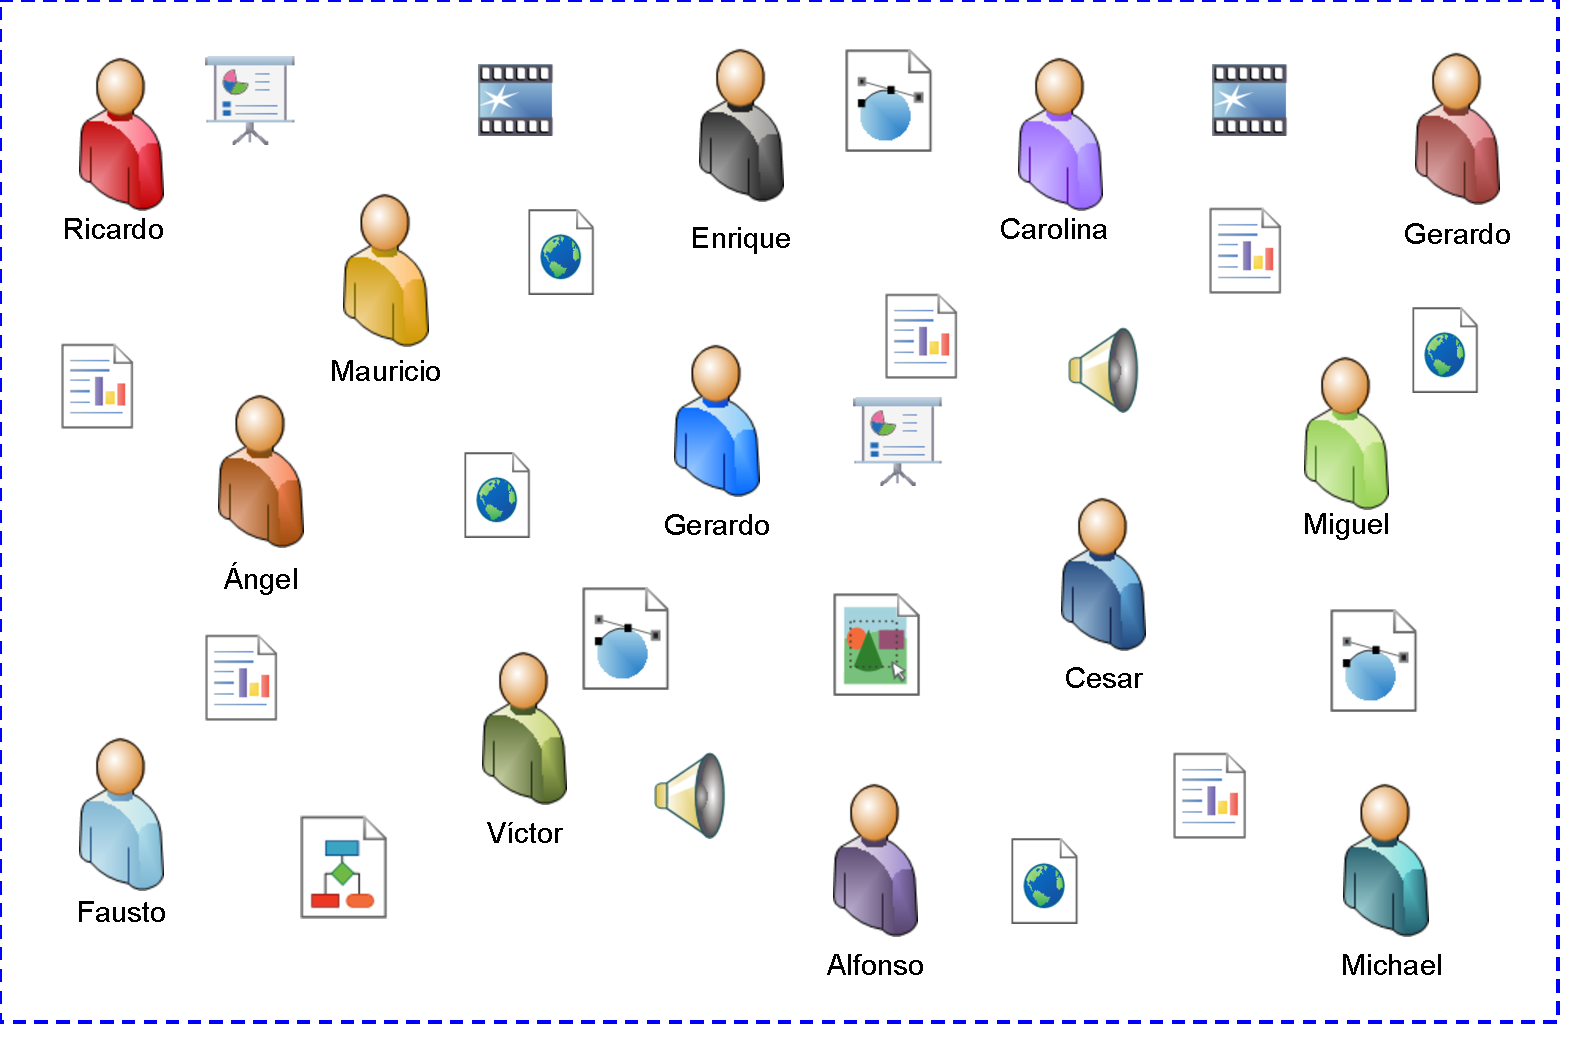
\includegraphics[scale=0.19]{EjemploMC} 
	}
	\end{figure}
	%%%%%%%%%%%%%%%%%%%%%%%
\end{frame}

\subsection{Integraci�n de la informaci�n de los recursos de informaci�n}
\begin{frame}
	\frametitle{Integraci�n de la informaci�n de los recursos de informaci�n}
	\begin{block}{Definici�n}
	\justifying
	\small La b�squeda y recuperaci�n significativa de informaci�n existente en los recursos de informaci�n para responder una consulta dada por un usuario.
	\end{block}
	
	\begin{exampleblock}{Etapas}
	\begin{enumerate}[<+-| alert@+>]
	\item \justifying \small Representar el conocimiento e informaci�n de los \textit{recursos de informaci�n}.
	\item \justifying \small Buscar y recuperar informaci�n, mediante la interrogaci�n de la representaci�n de conocimiento (modelo).
	\end{enumerate}
	\end{exampleblock}
	
	\begin{figure}
	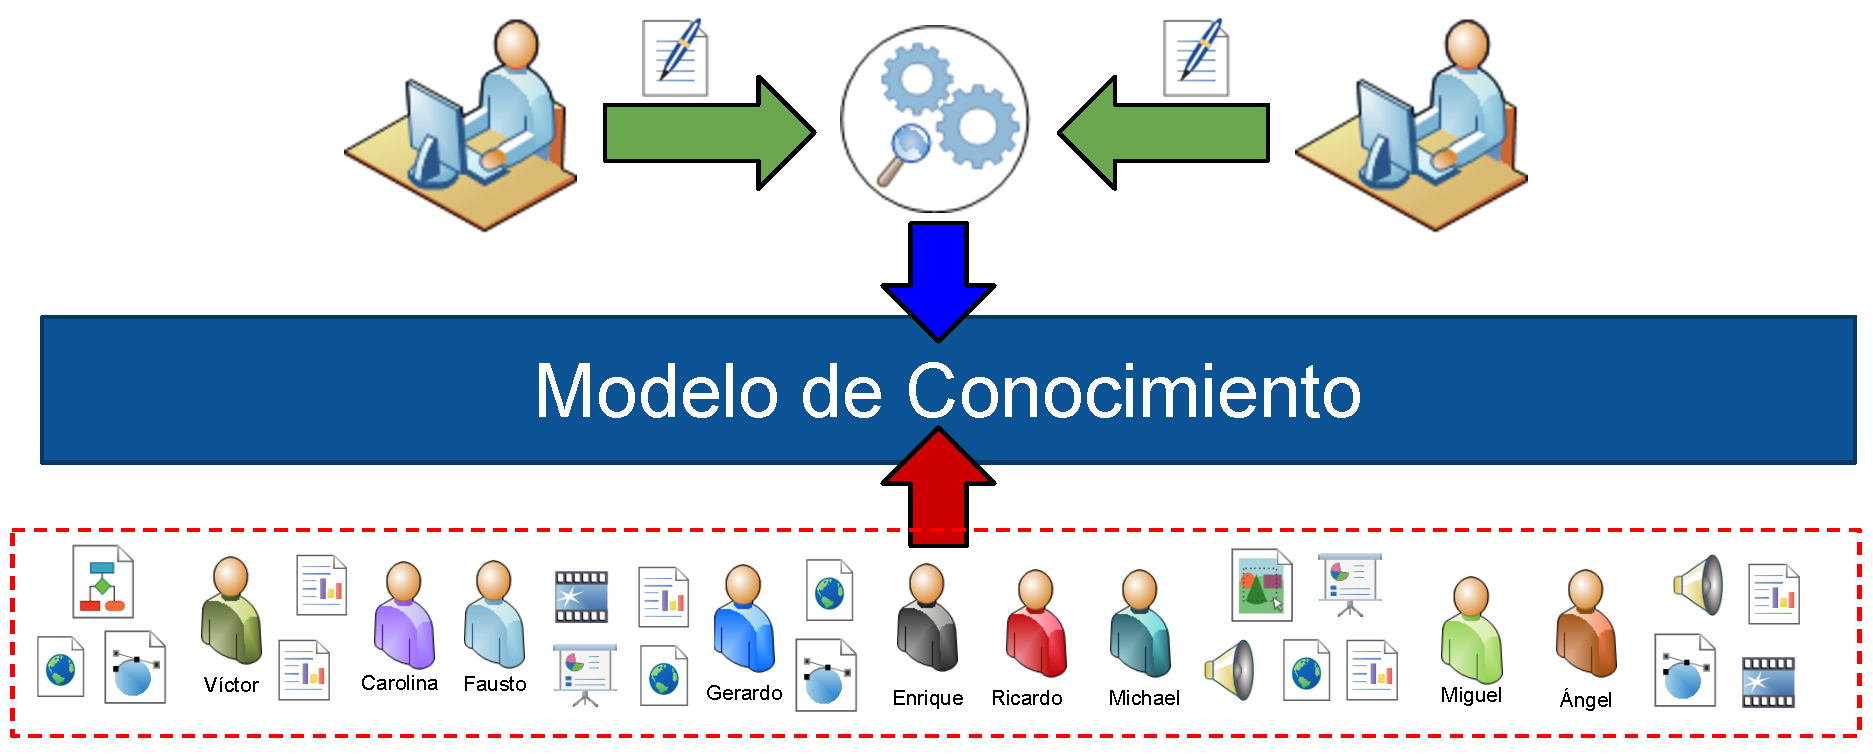
\includegraphics[scale=0.24]{IntegracionSemantica} 
	\end{figure}
\end{frame}

\subsection{Tecnolog�as Sem�nticas}
\begin{frame}
	\frametitle{Tecnolog�as Sem�nticas}
	\begin{block}{Definici�n}
	\justifying 
	\textit{Un conjunto de metodolog�as, lenguajes, aplicaciones, herramientas y est�ndares para suministrar u obtener el significado de las palabras, informaci�n y las relaciones entre �stos}. \begin{scriptsize}\cite{SemTecRetr}\end{scriptsize}
	\end{block}
	
	\begin{figure}
	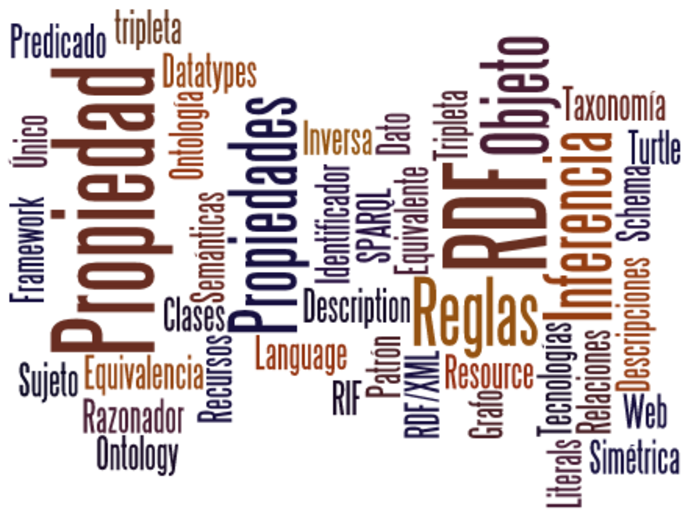
\includegraphics[scale=0.42]{TSWords} 
	\end{figure}
\end{frame}

\subsection{Integraci�n sem�ntica de recursos de informaci�n}
\begin{frame}
	\frametitle{Integraci�n sem�ntica de recursos de informaci�n}
	\begin{figure}
	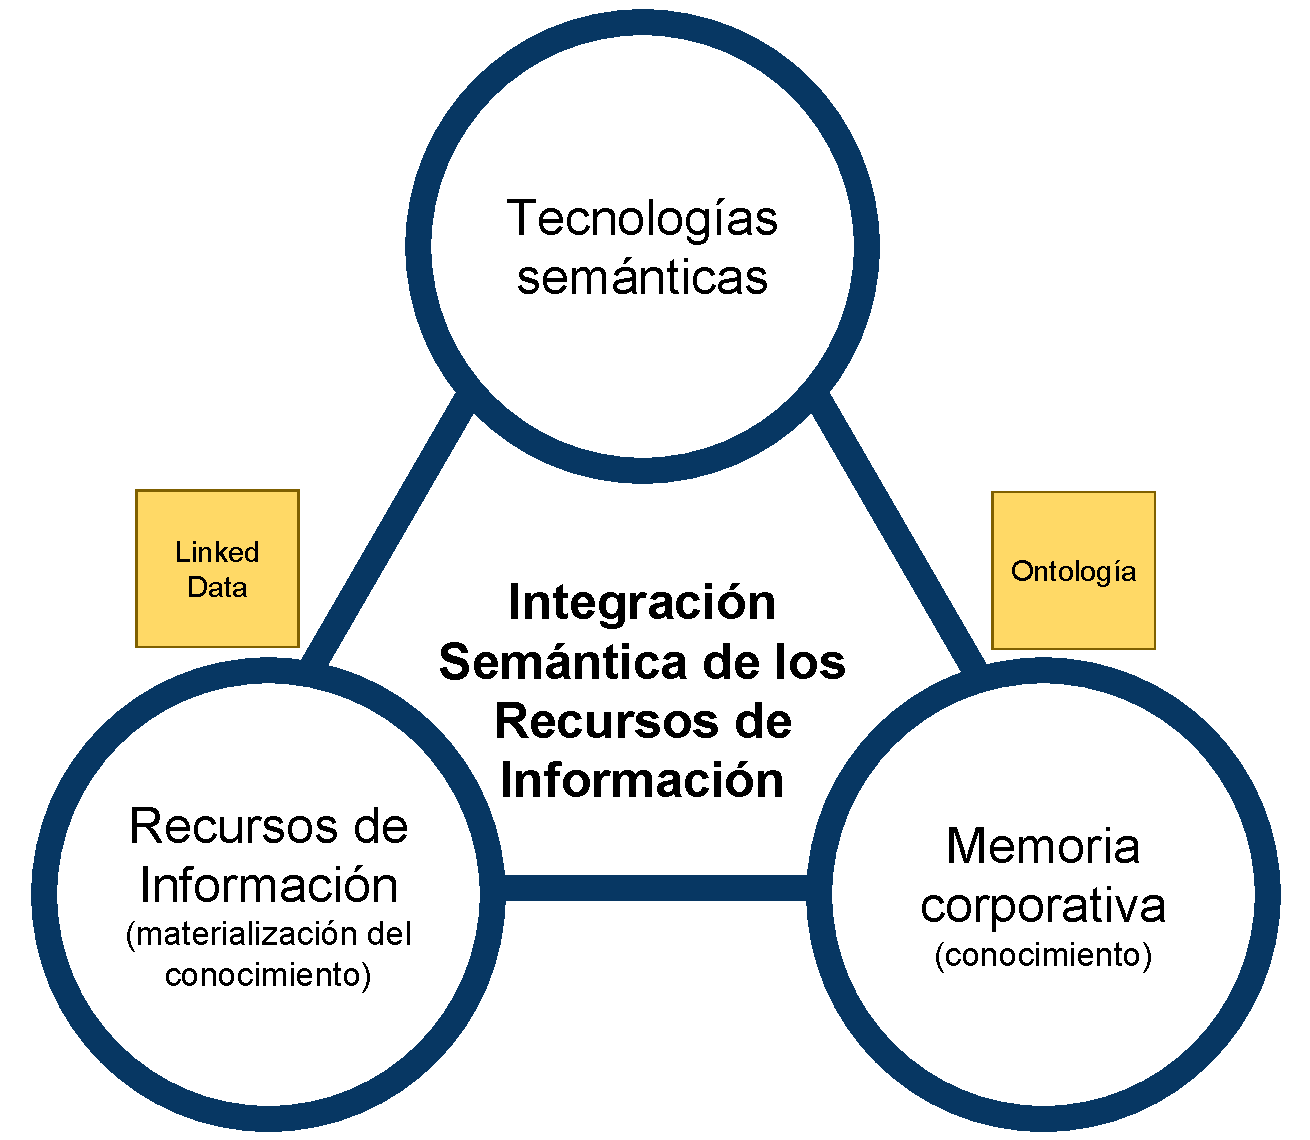
\includegraphics[scale=0.38]{ISRIMC} 
	\end{figure}
\end{frame}

\subsection{Estado del Arte}
\begin{frame}
	\frametitle{Estado del Arte}
	\begin{block}{Ejes claves}
	\begin{enumerate}
	\item \justifying Integraci�n de la informaci�n a partir del uso de tecnolog�as sem�nticas.
	\item \justifying B�squeda, recuperaci�n y publicaci�n de la informaci�n desde una ontolog�a.
	\item \justifying Gesti�n de una memoria corporativa.
	\end{enumerate}
	\end{block}
	
	\begin{figure}
	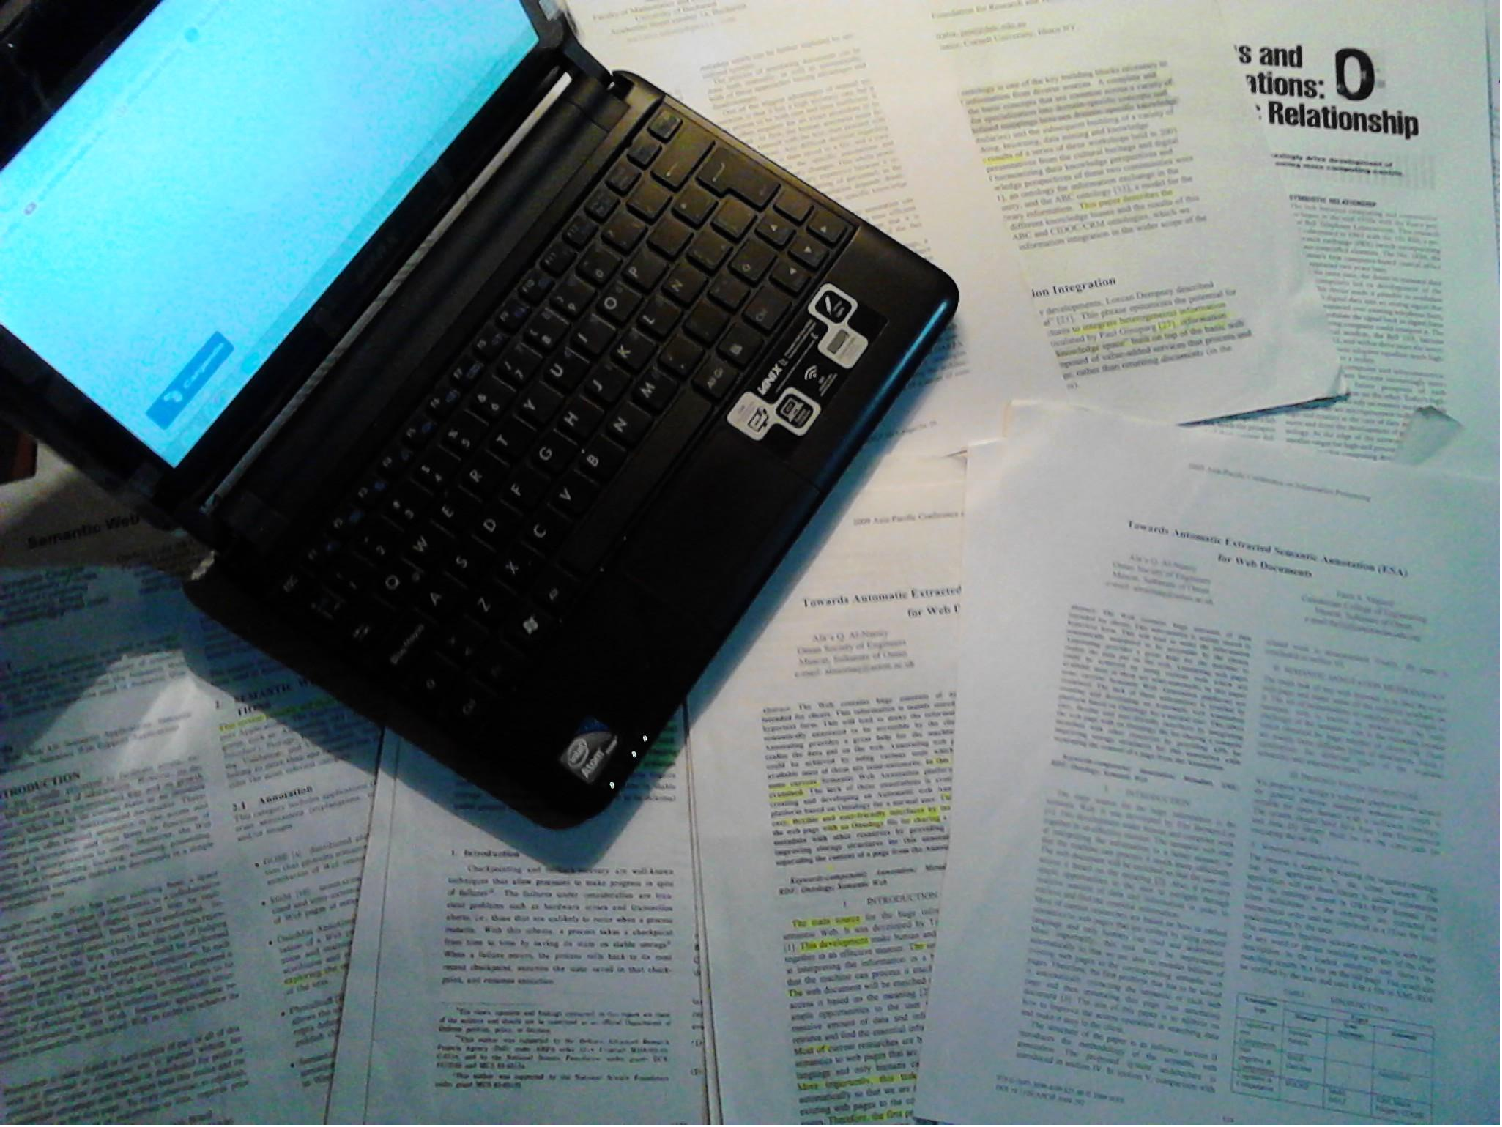
\includegraphics[scale=0.15]{EstadoArte} 
	\end{figure}
\end{frame}

\begin{frame}
	\frametitle{Comparativa}
	\begin{figure}
	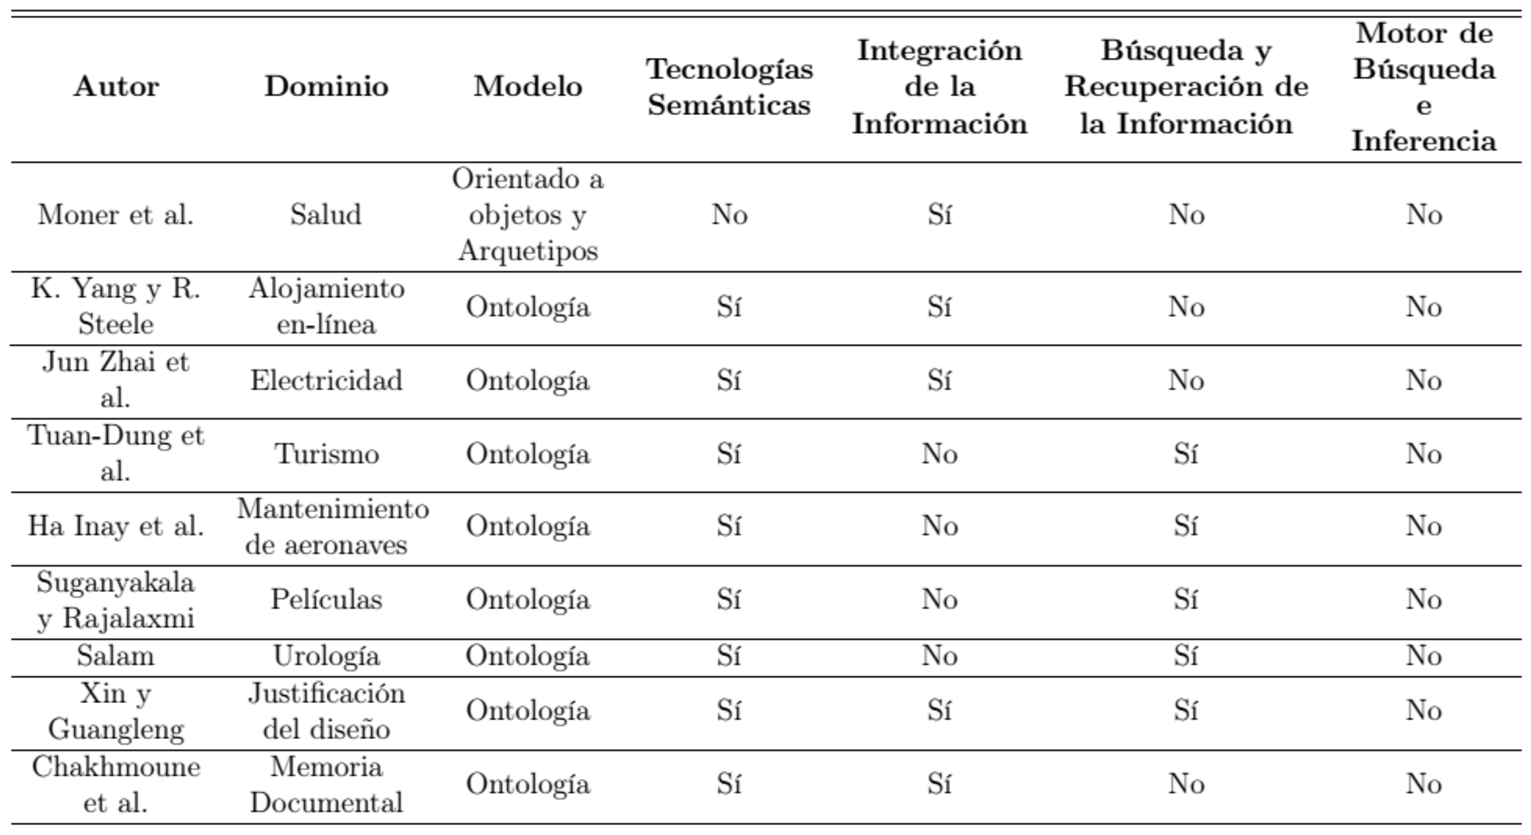
\includegraphics[scale=0.42]{TablaEOA} 
	\end{figure}
\end{frame}
\section{Problema}
\begin{frame}
	\frametitle{Problema} 
	\begin{exampleblock}{Pregunta investigaci�n}
	\justifying 
	\small �El \textit{conocimiento impl�cito} es un factor importante para la obtenci�n de \textit{recursos de informaci�n pertinentes} a una consulta?
	\end{exampleblock}
	
	\begin{figure}
	
\includegraphics[scale=0.28]{PreguntaInv} 
	\end{figure}
	
	\begin{block}{Hip�tesis}
	\justifying 
	\small El uso de las \textit{tecnolog�as sem�nticas} es adecuado para lograr la \textit{integraci�n sem�ntica} de \textit{recursos de informaci�n} en una \textit{memoria corporativa}.
	\end{block}
\end{frame}

\subsection{Objetivo General}
\begin{frame}
	\frametitle{Objetivo General}
	\begin{alertblock}{}
	\justifying 
	Contribuir a la \textit{integraci�n sem�ntica} de los \textit{recursos de informaci�n} existentes en \textit{una memoria corporativa}, mediante el uso de las \textit{tecnolog�as sem�nticas}.
	\end{alertblock}
\end{frame}

\subsection{Objetivos}
\begin{frame}
	\frametitle{Objetivos Particulares} 
	\begin{enumerate}
	\item \justifying \small Proponer un \textbf{marco de referencia} para la \textit{integraci�n sem�ntica} de los \textit{recursos de informaci�n} existentes en una memoria corporativa.
	\item \justifying \small Proponer un \textbf{modelo sem�ntico} que represente el \textit{conocimiento expl�cito e impl�cito} existente en los \textit{recursos de informaci�n}.
	\item \justifying \small Implementar un \textbf{prototipo} que permita a los usuarios buscar y recuperar \textit{recursos de informaci�n} existentes en una memoria corporativa, as� como visualizar las caracterizaciones de estos recursos.
	\end{enumerate}
\end{frame}

%\subsection{Metodolog�a}
%\begin{frame}
%	\frametitle{Metodolog�a I}
%	\begin{block}{Marco de Referencia}
%	\begin{enumerate}
%	\item \justifying \small Identificar los principales \textit{casos de uso}.
%	\item \justifying \small Evaluar las \textit{herramientas sem�nticas}.
%	\item \justifying \small Componer la \textit{memoria corporativa} de RyT.
%	\end{enumerate}
%	
%	\begin{exampleblock}{Modelo Sem�ntico}
%	\begin{enumerate}
%	\setcounter{enumi}{3}
%	\item \justifying \small Representar el \textit{conocimiento expl�cito} de los \textit{recursos de informaci�n} en un \textit{modelo sem�ntico} (ontolog�a).
%	\item \justifying \small Enriquecer el \textit{modelo sem�ntico} con \textit{reglas de inferencia}.
%	\end{enumerate}
%	\end{exampleblock}
%	
%	\begin{enumerate}
%	\setcounter{enumi}{5}
%	\item \justifying \small Encontrar las principales \textit{consultas}.
%	\item \justifying \small Hacer expl�cito el conocimiento impl�cito.
%	\item \justifying \small Buscar y recuperar informaci�n en el modelo inferido.
%	\end{enumerate}
%	\end{block}
%\end{frame}
%
%\begin{frame}
%	\frametitle{Metodolog�a II}	
%	\begin{block}{Prototipo de interfaz gr�fica de usuario}	
%	\begin{enumerate}
%	\setcounter{enumi}{8}
%	\item \justifying \small Construir el \textit{prototipo de interfaz de usuario} para la (b�squeda y navegaci�n) de los usuarios en un modelo sem�ntico.
%	\end{enumerate}
%	\end{block}
%	
%	\begin{block}{Evaluaci�n}
%	\begin{enumerate}
%	\setcounter{enumi}{9}
%	\item \justifying \small Evaluar la calidad de los resultados con y sin inferencia.
%	\item \justifying \small Evaluar los \textit{tiempos promedios} de consulta sobre modelos con/sin inferencia.
%	\end{enumerate}
%	\end{block}
%\end{frame}

\section{Metodolog�a}
\begin{frame}
	\frametitle{Integraci�n Sem�ntica mediante tecnolog�as sem�nticas}
	\begin{block}{Metodolog�a}
		\begin{enumerate}%[<+-| alert@+>]
		\item \justifying Representar las caracter�sticas y/o relaciones de los \textit{recursos de informaci�n}, para construir un modelo sem�ntico.
		\item \justifying Introducir \textit{reglas de inferencia} en el modelo, para obtener conocimiento impl�cito.
		\item \justifying Buscar y recuperar conocimiento en el modelo sem�ntico para responder un conjunto consultas que lleven a \textit{recursos de informaci�n}.
		\end{enumerate}
	\end{block}
\end{frame}

\begin{frame}
	\frametitle{Arquitectura}	
	\begin{figure}
	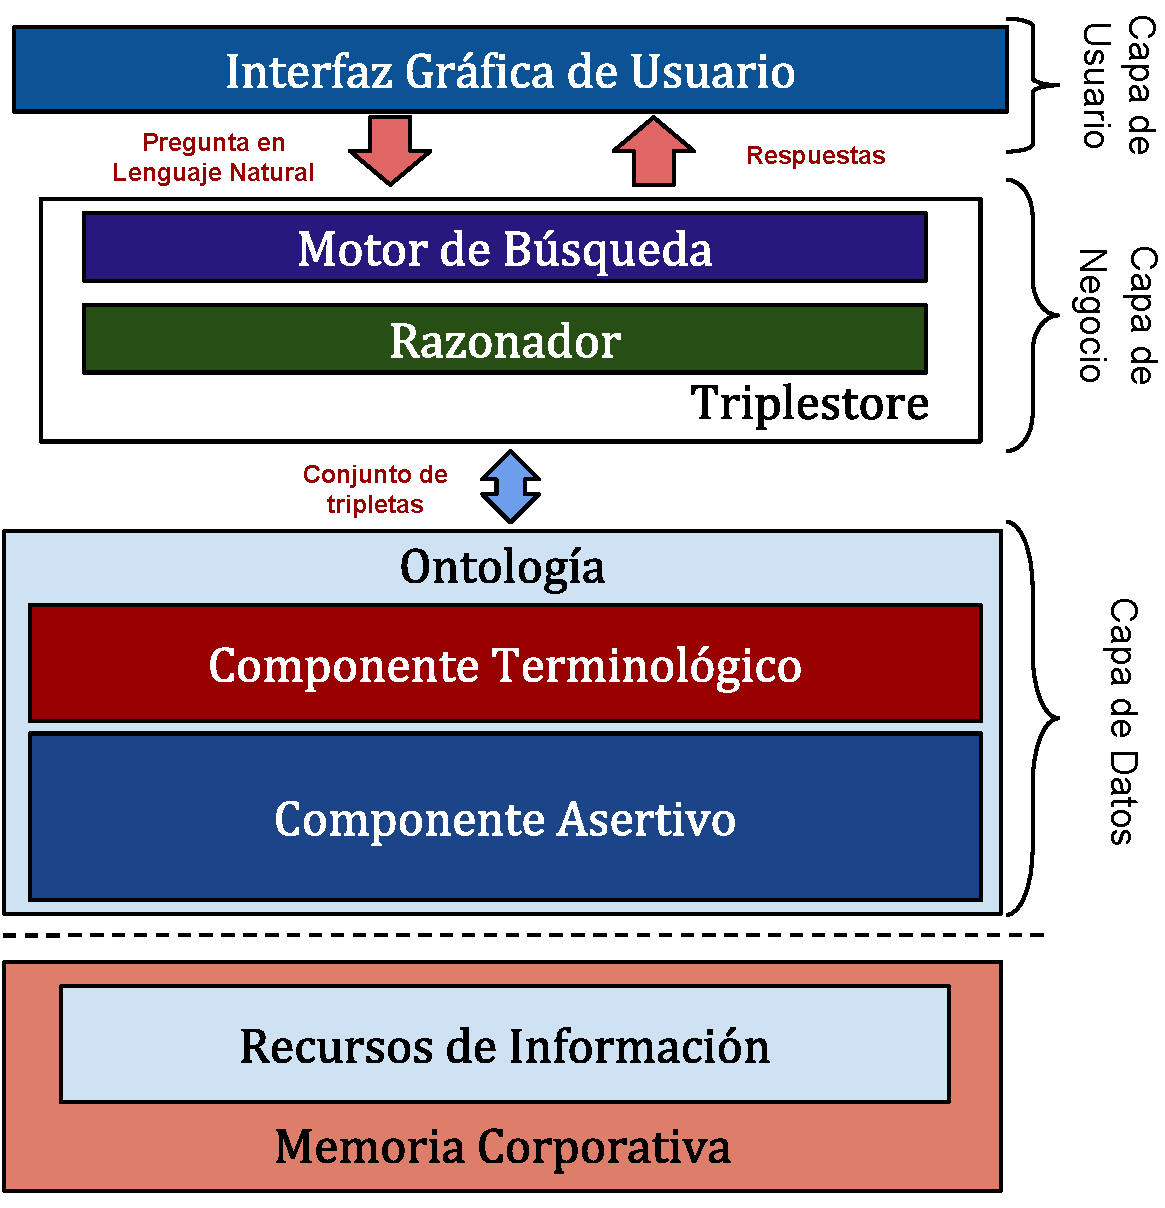
\includegraphics[scale=0.3]{Arquitectura} 
	\end{figure}
\end{frame}

\subsection{Representaci�n del conocimiento}
\begin{frame}
	\frametitle{Representaci�n del conocimiento}
	
	\begin{block}{Resource Description Framework}
	\justifying 
	\small Es un marco gen�rico para describir el conocimiento e informaci�n expl�cita de los recursos mediante sus caracter�sticas y relaciones.
	\end{block}
	
	\begin{figure}
	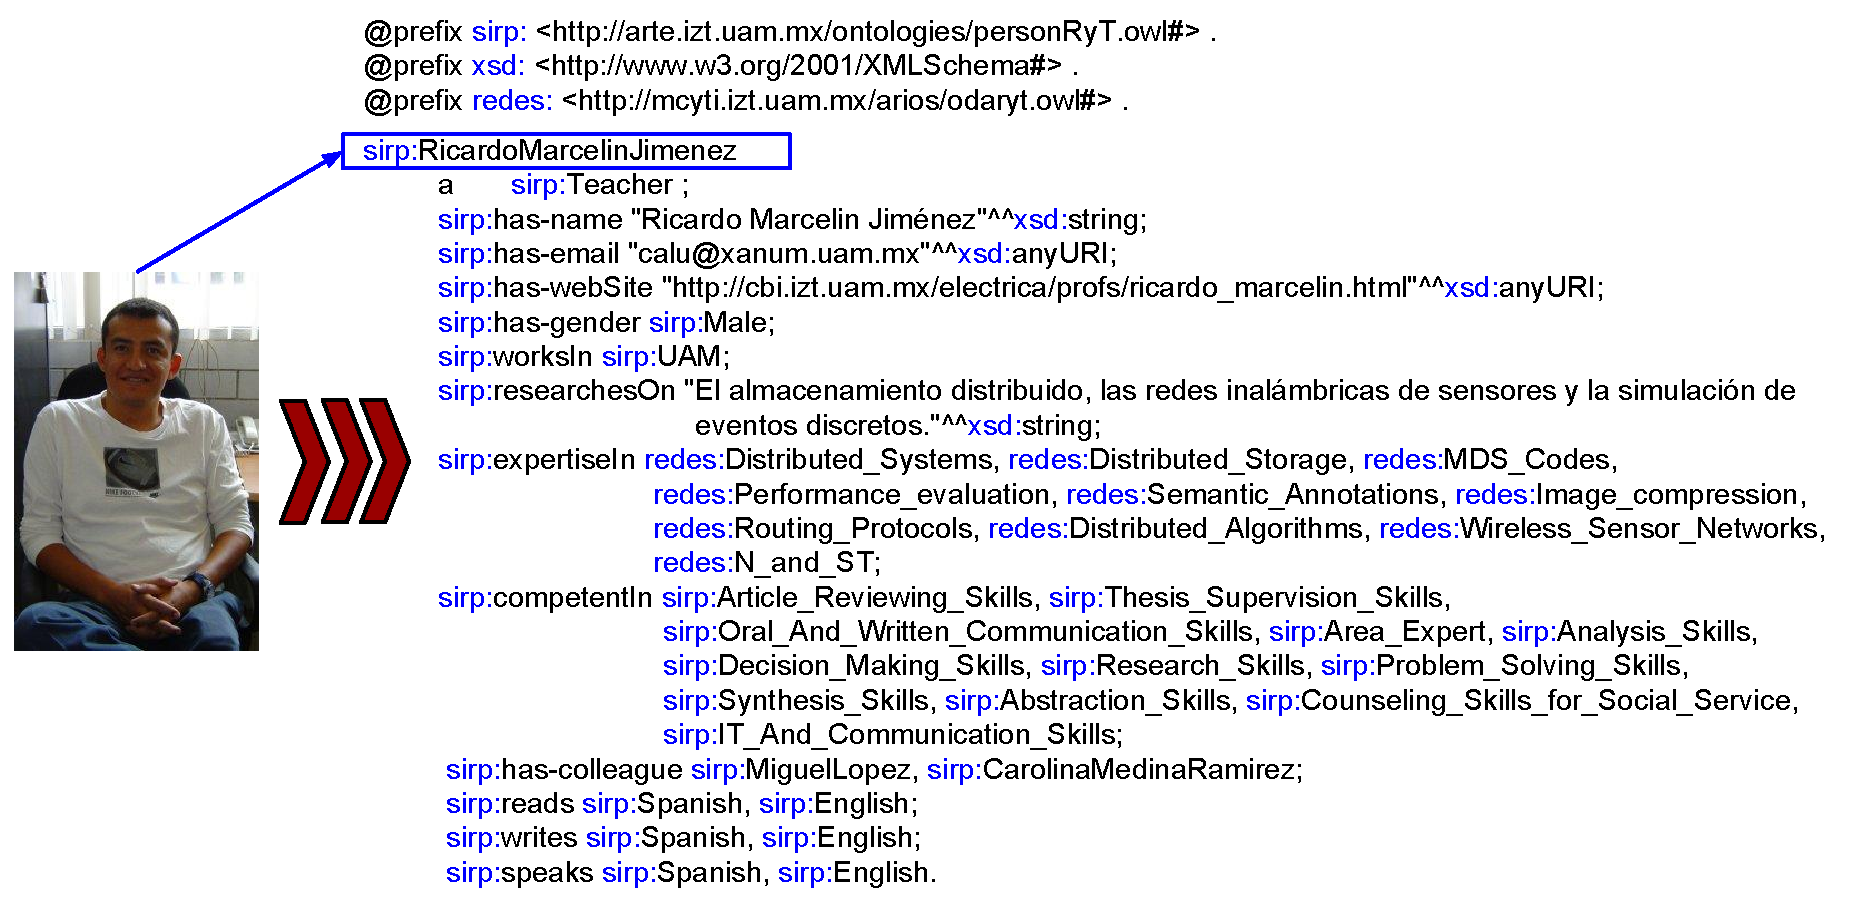
\includegraphics[scale=0.30]{Person2RDF}
	\end{figure}
\end{frame}

%\begin{frame}
%	\frametitle{Representar el conocimiento e informaci�n mediante el est�ndar RDF}
%	\begin{figure}
%	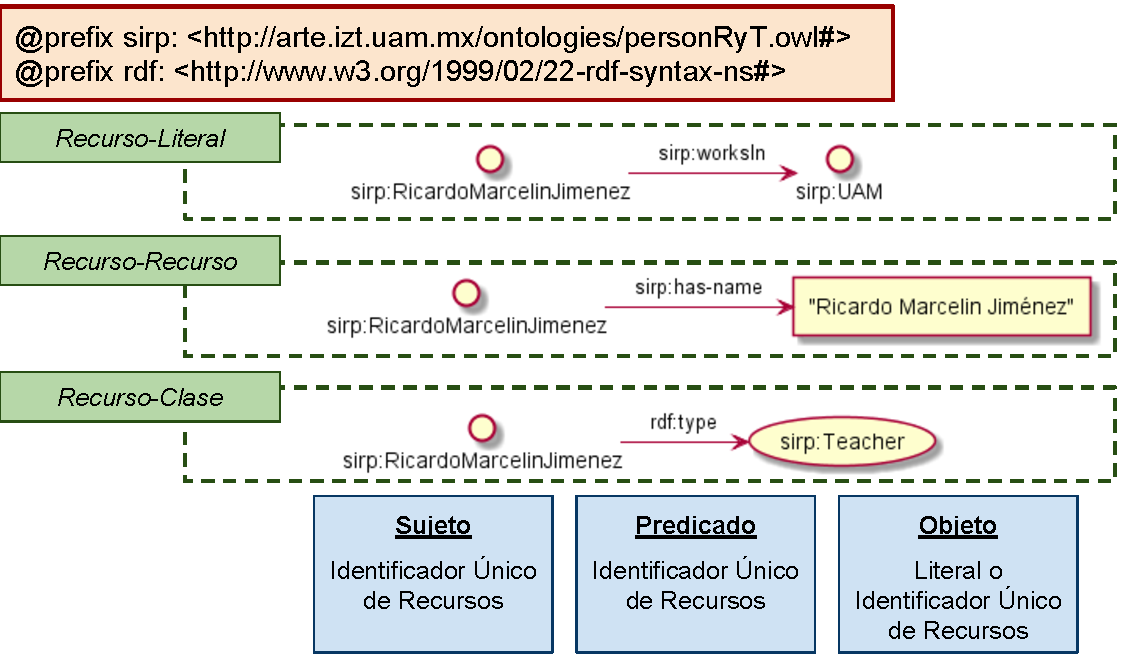
\includegraphics[scale=0.45]{Tripletas} 
%	\end{figure}
%\end{frame}

\begin{frame}
	\frametitle{Grafo RDF}
	\begin{figure}
	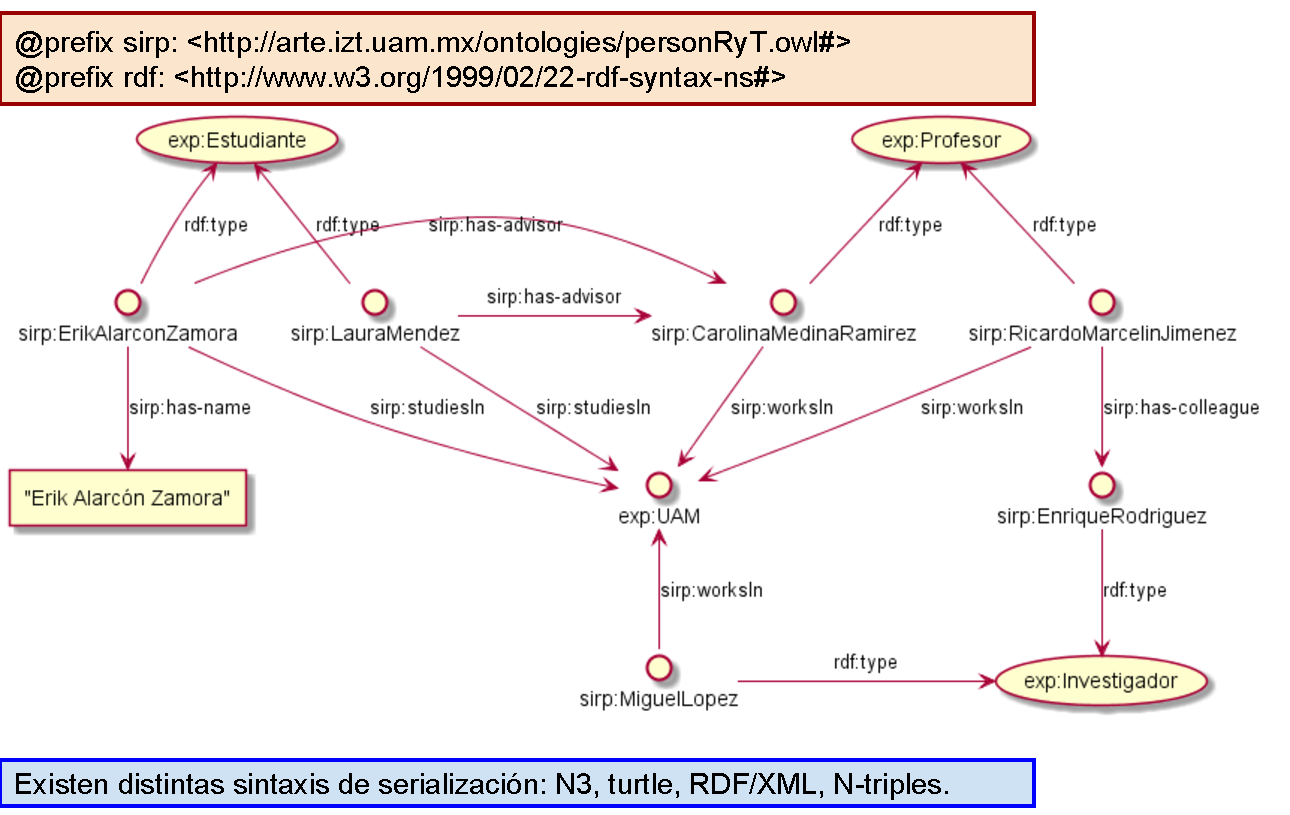
\includegraphics[scale=0.48]{GrafoRDF} 
	\end{figure}
\end{frame}

\subsection{Enriquecer el conocimiento en el modelo sem�ntico}
\begin{frame}
	\frametitle{Introducir reglas de inferencia}	
	\begin{block}{Reglas de inferencia o Axiomas}
	\justifying 
	\small Son expresiones para enriquecer un grafo RDF con conocimiento impl�cito de las clases y relaciones.
	\end{block}
	
	\begin{figure}[htbp]
	\centering
	\subfigure[Jerarqu�a de Clases]{
	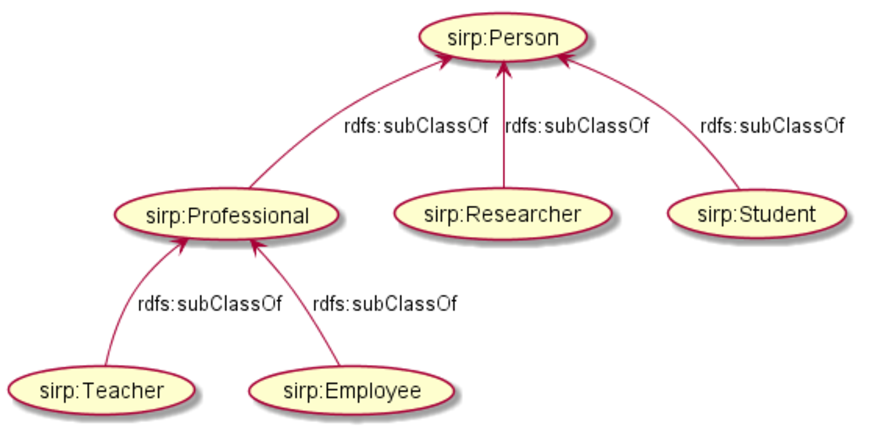
\includegraphics[scale=0.37]{HerenClassCartComp} 
	}
	\subfigure[Dominio y rango]{
	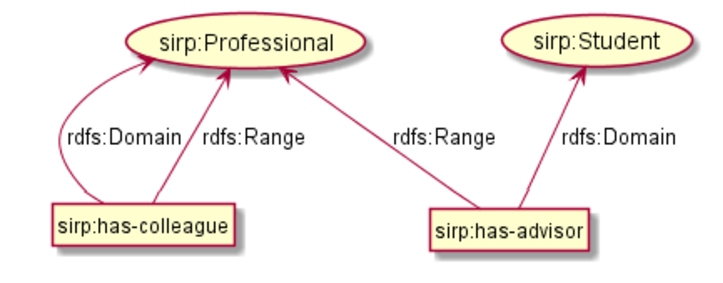
\includegraphics[scale=0.37]{exAxDyRPer} 
	}
	\end{figure}
\end{frame}

\begin{frame}
	\frametitle{Emplear un programa para inferir conocimiento}	
	\begin{block}{Razonador}
	\justifying 
	\small Es un programa que deduce conocimiento a partir de los axiomas y declaraciones expl�citas en un modelos sem�ntico.
	\end{block}
	
	\begin{figure}
	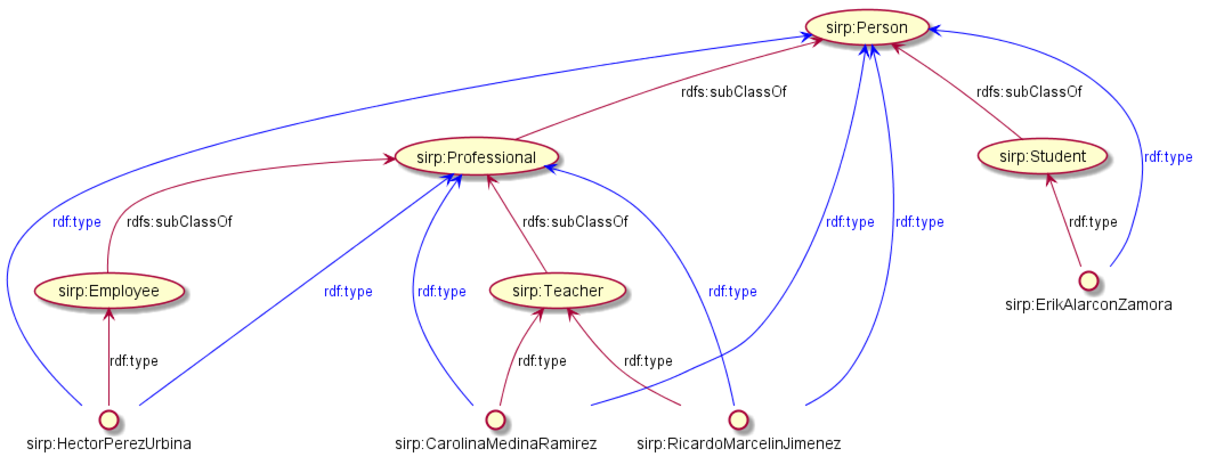
\includegraphics[scale=0.50]{EjmpInfSubClass}
	\end{figure}
\end{frame}

\begin{frame}
	\frametitle{Emplear un programa para inferir conocimiento}	
	\begin{figure}
	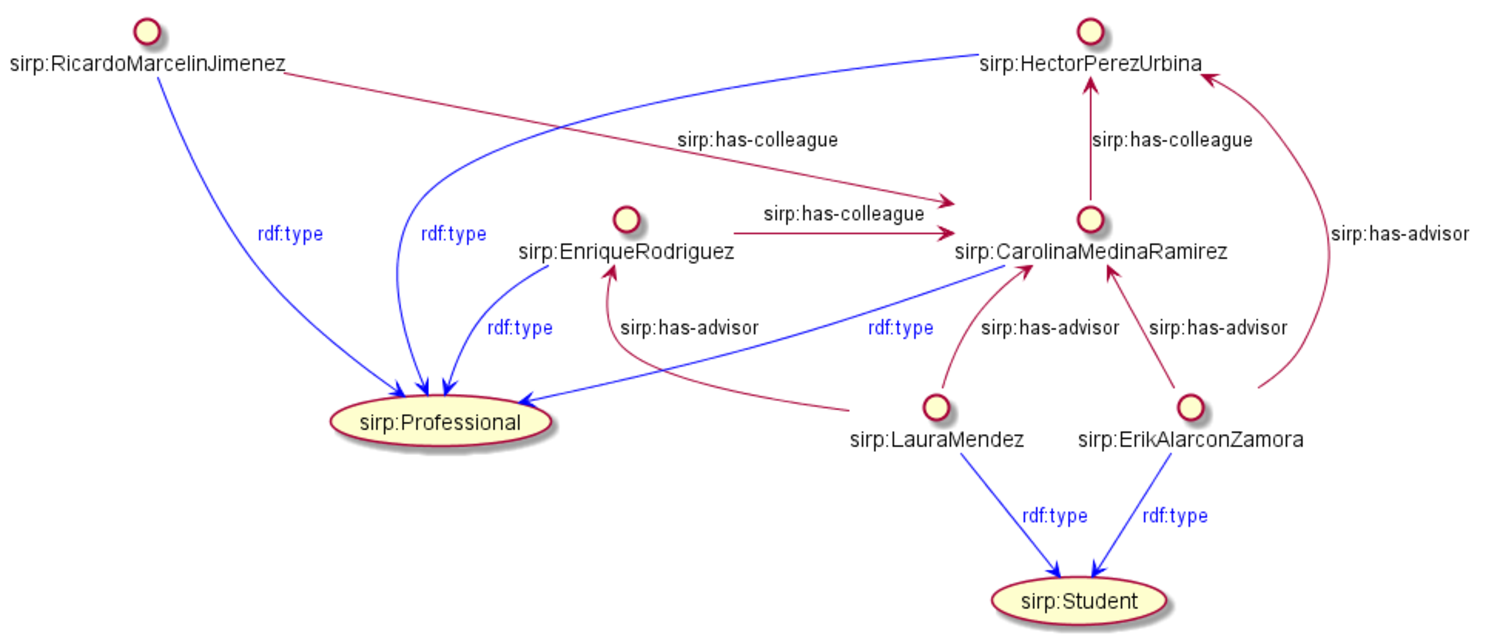
\includegraphics[scale=0.45]{exInfDyRPer}
	\end{figure}
\end{frame}

\subsection{Buscar y recuperar la informaci�n en el modelo sem�ntico}
\begin{frame}
	\frametitle{Buscar y recuperar la informaci�n en el modelo sem�ntico}
%	\begin{block}{Objetivo}
%	\justifying
%	La b�squeda y recuperaci�n de la informaci�n para responder las preguntas o necesidades informativas de los usuarios del �rea de Redes y Telecomunicaciones (RyT).
%	\end{block}
	
	\begin{block}{SPARQL}
	\justifying 
	Es un lenguaje de consulta para la recuperaci�n de informaci�n en un grafo RDF.
	\end{block}
	
	\begin{figure}
	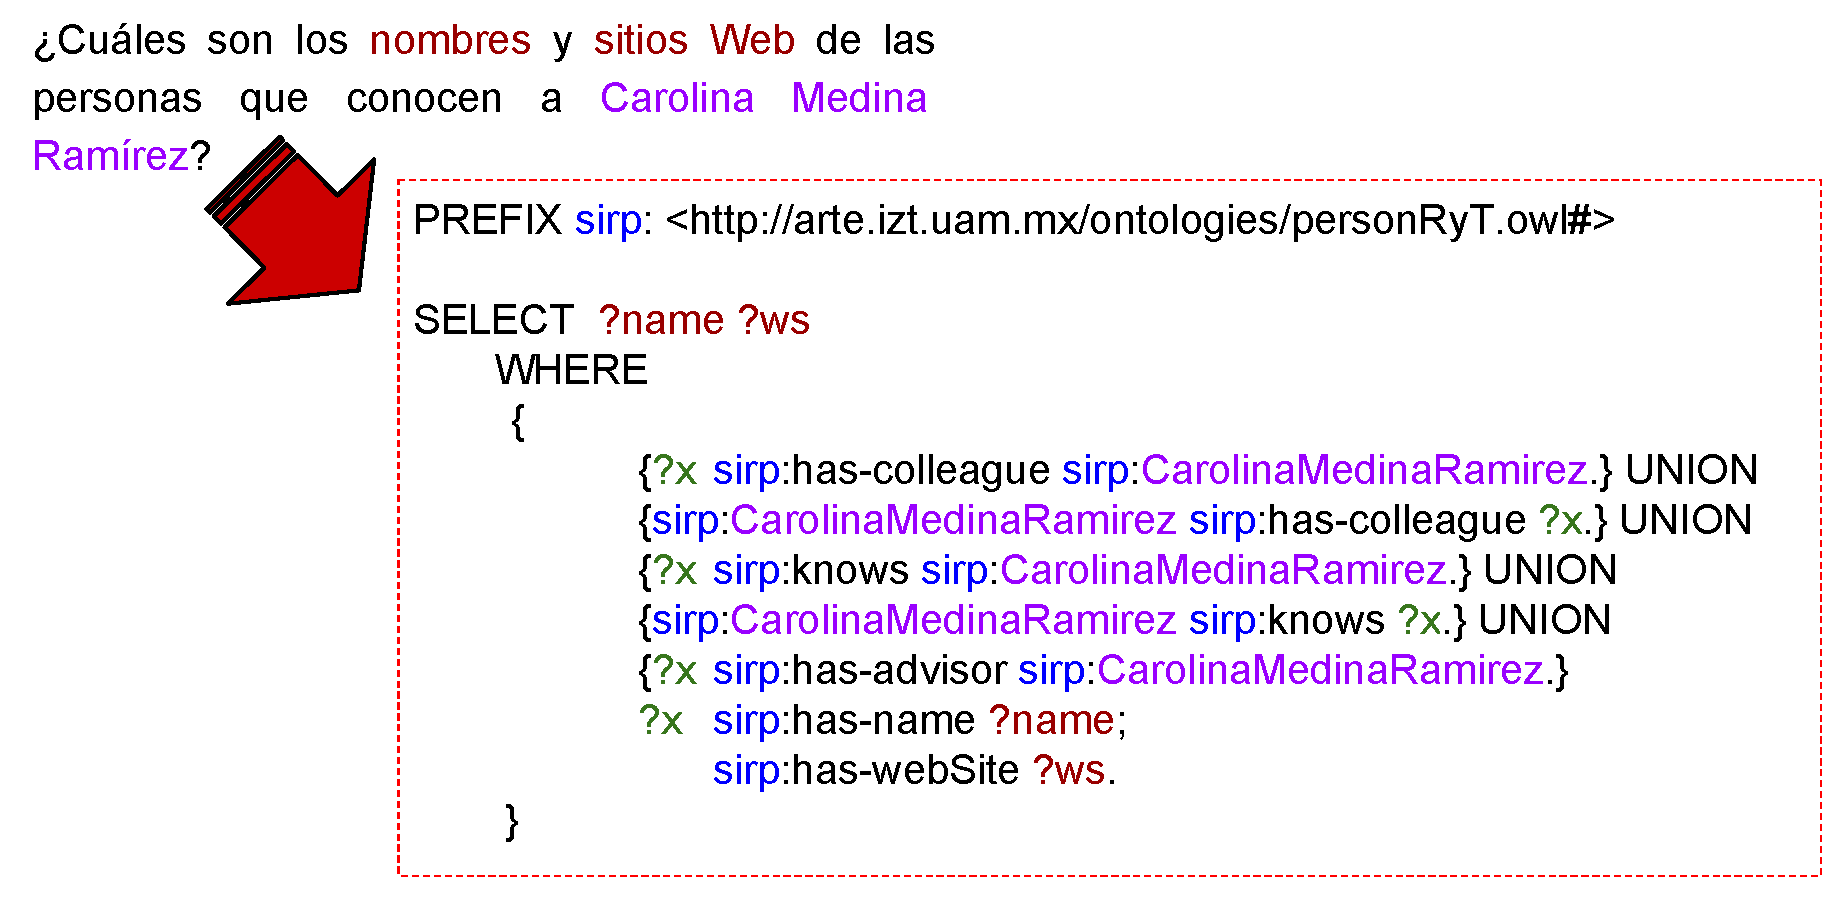
\includegraphics[scale=0.32]{q2rqlSR}
	\end{figure}
\end{frame}

\subsection{Herramientas para la Integraci�n Sem�ntica}
\begin{frame}
	\frametitle{Herramientas para la Integraci�n Sem�ntica}
	\begin{block}{Descriptor Sem�ntico de Recursos}
	\justifying
	\small Herramienta para crear y almacenar tripletas RDF, en varias sintaxis de serializaci�n, a partir de la informaci�n expl�cita de los recursos de informaci�n. \textbf{\textit{OntoMat Annotizer}}, \textbf{\textit{MnM}}, \textbf{\textit{GATE}} y \textbf{\textit{Aktive Media}}.
	\end{block}
	
	\begin{block}{Editor de Ontolog�as}
	\justifying
	\small Herramienta que proporciona una serie de interfaces amigables para la construcci�n y mantenimiento de ontolog�as. \textbf{\textit{Prot�g�}}, \textbf{\textit{pOWL}}, \textbf{\textit{TopBraid Composer}} y \textbf{\textit{SWOOP}}.
	\end{block}
	
	\begin{block}{Triplestore}
	\justifying
	\small Programa para el almacenamiento e indexaci�n de tripletas RDF, con el fin de permitir la consulta eficiente de informaci�n sobre estas tripletas. \textbf{\textit{Jena}}, \textbf{\textit{Stardog}}, \textbf{\textit{4store}} y \textbf{\textit{Sesame}}.
	\end{block}
\end{frame}

\subsection{Construir un Prototipo (Aplicaci�n)}
\begin{frame}%[allowframebreaks]
	\frametitle{Construir un Prototipo (Aplicaci�n)}
	\begin{block}
	\justifying
	\small El prototipo es una aplicaci�n Web que permite a los usuarios estructurar sus preguntas. �stas a trav�s del uso de un modelo sem�ntico recuperan recuperan los \textit{recursos de informaci�n}, as� como las caracter�sticas de los mismos.
	\end{block}
	
	\begin{figure}
	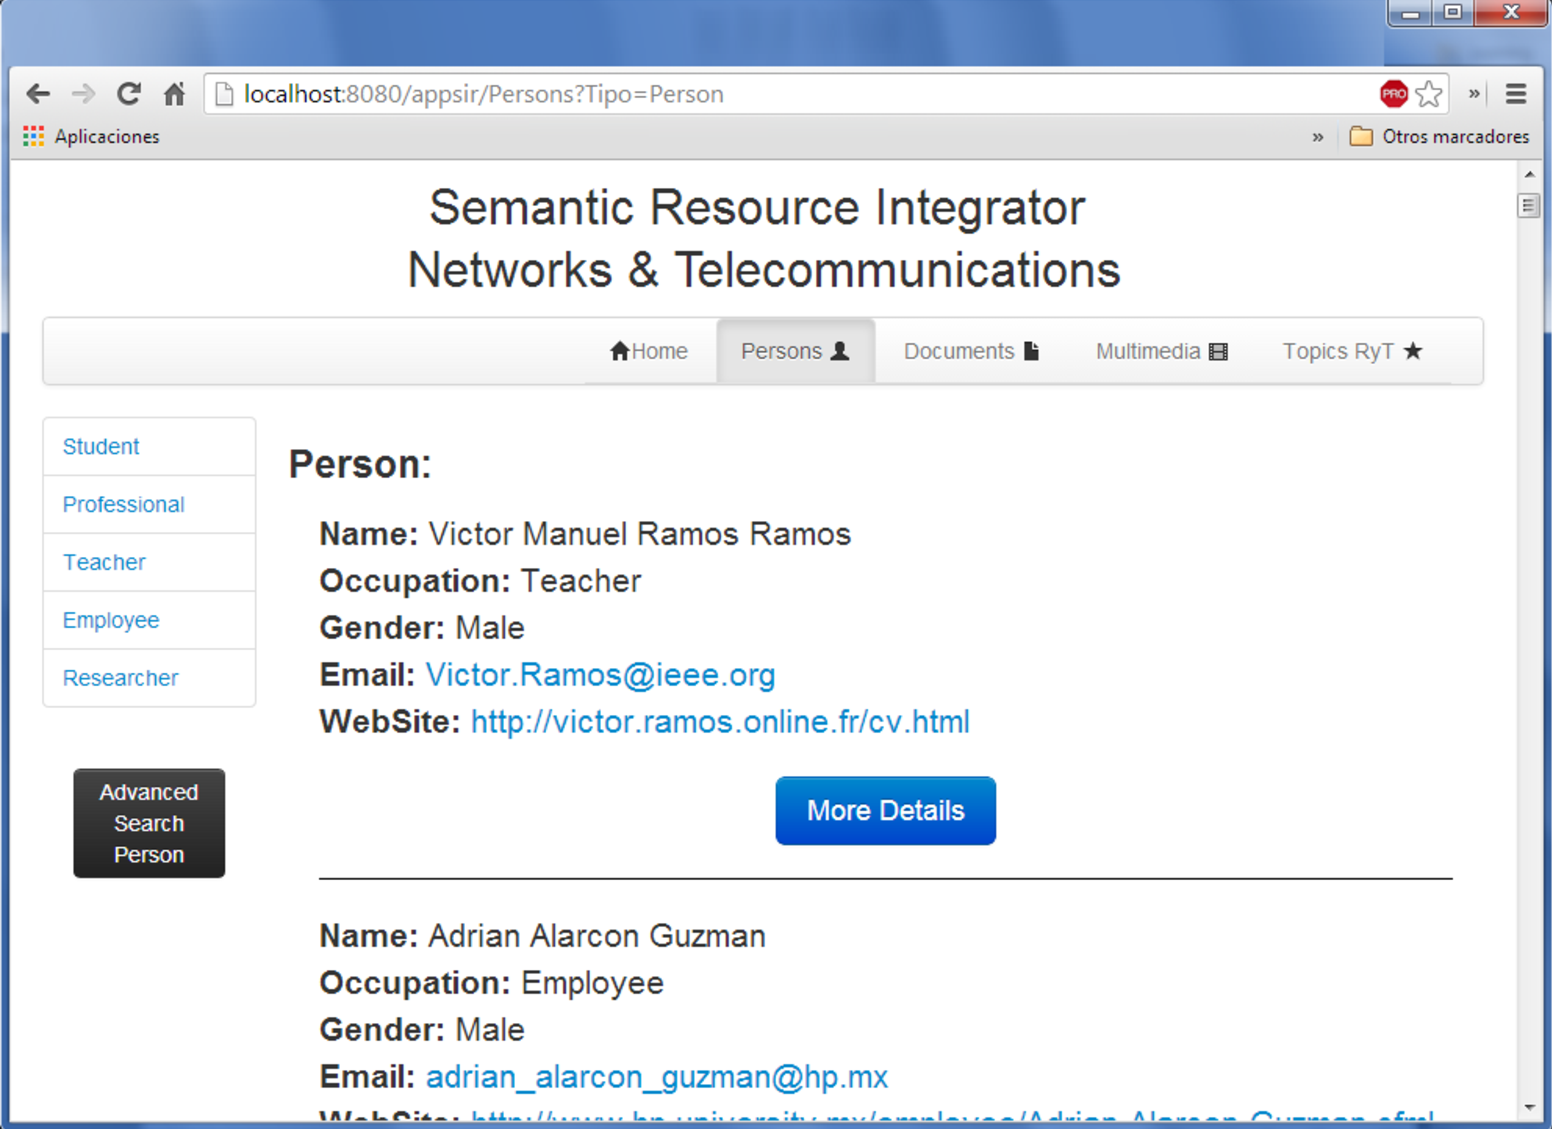
\includegraphics[scale=0.28]{IntWebNavPer} 
	\end{figure}
\end{frame}

\begin{frame}%[allowframebreaks]
	\frametitle{Construir un Prototipo (Aplicaci�n)}
	\begin{figure}
	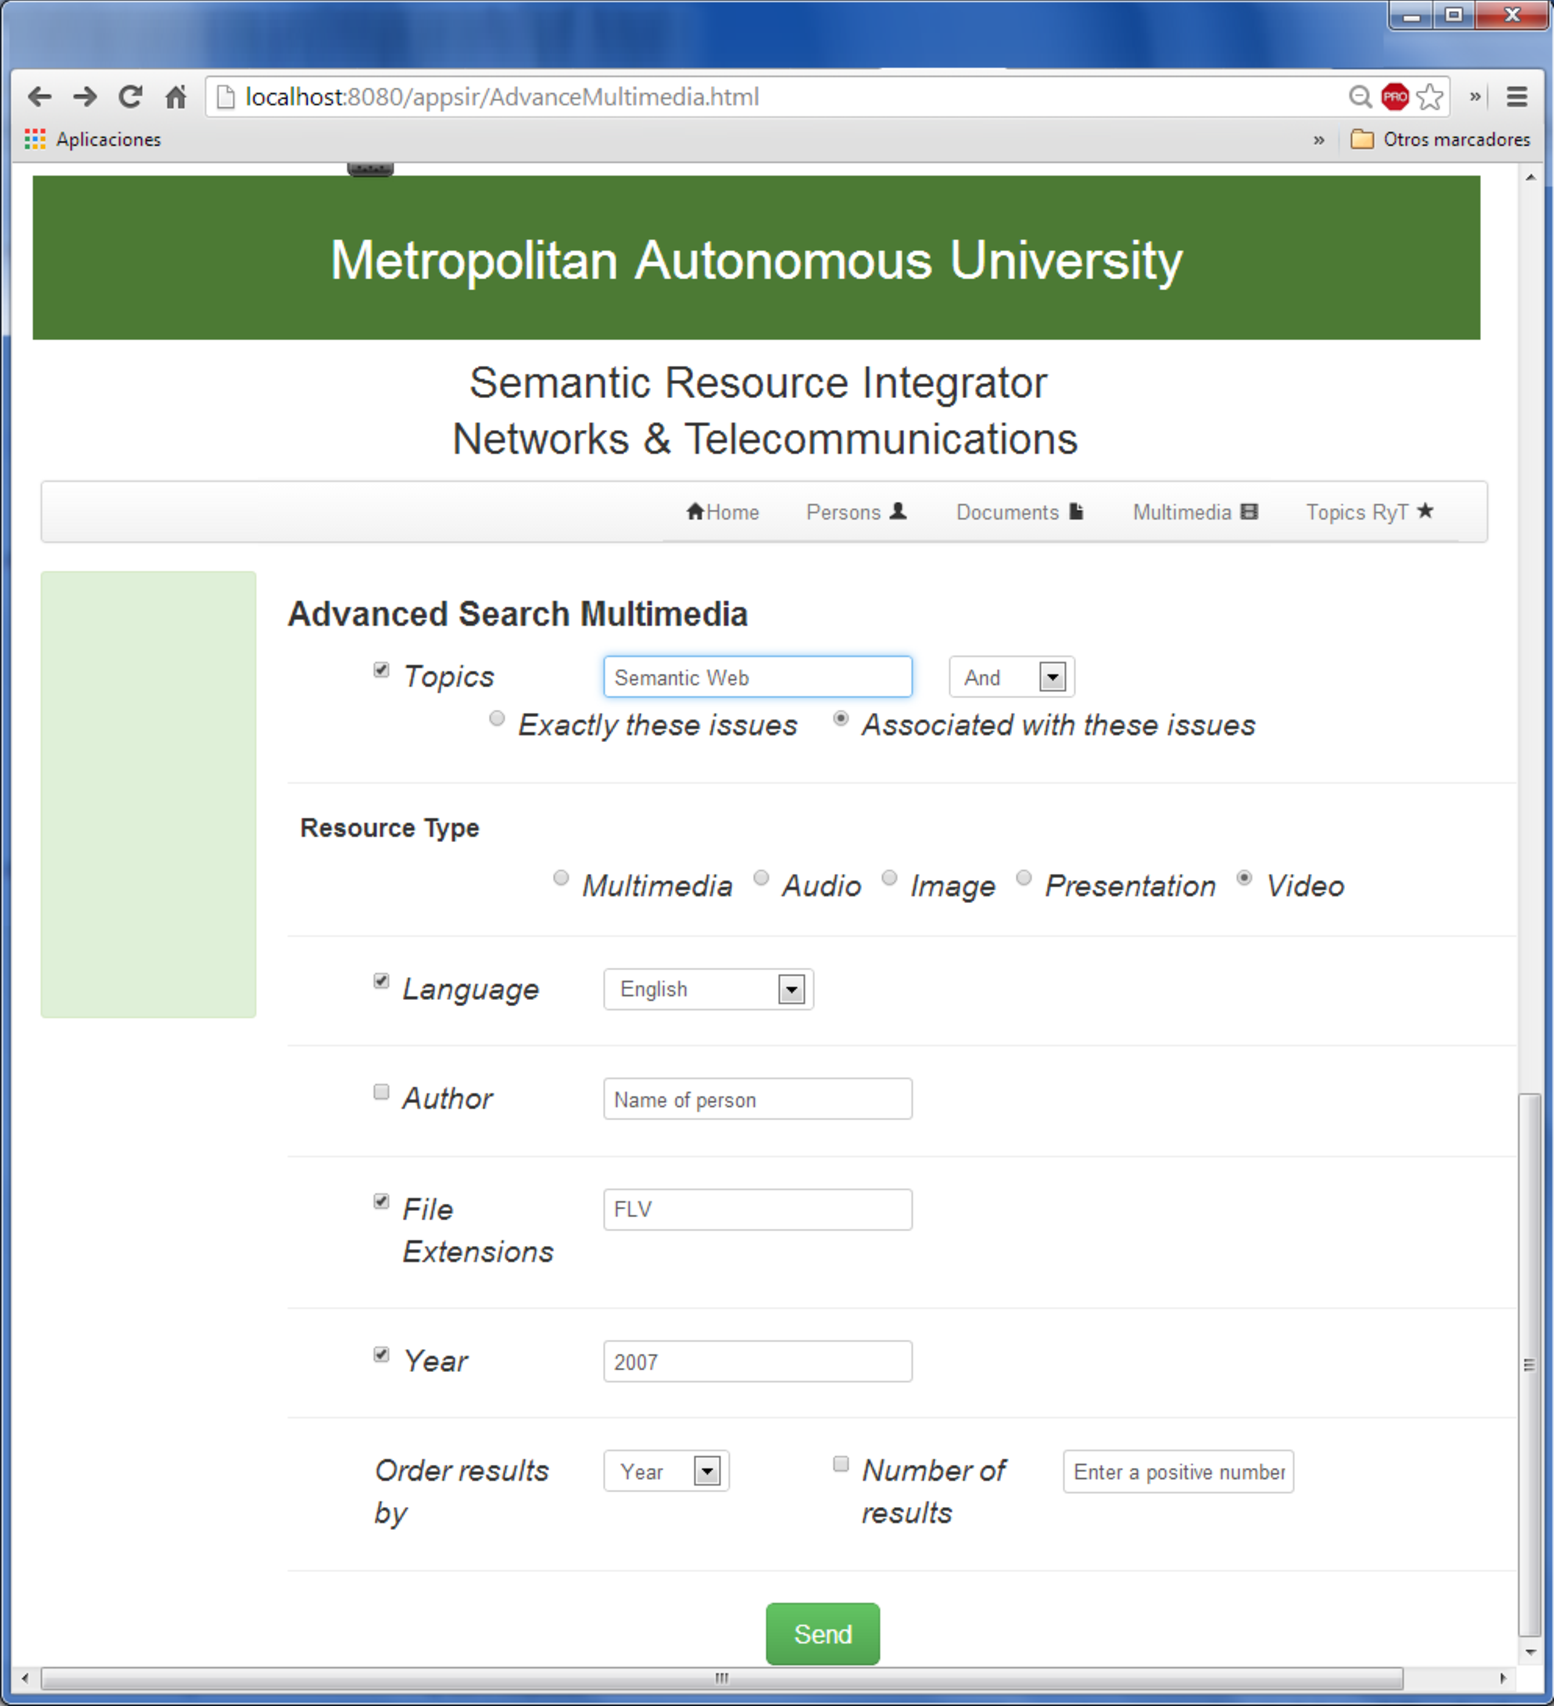
\includegraphics[scale=0.23]{FormBusMult} 
	\end{figure}
\end{frame}

\subsection{Evaluar la integraci�n sem�ntica}
\begin{frame}%[allowframebreaks]
	\frametitle{Evaluar la integraci�n sem�ntica}
	%%%%%%%%%%%%%%%%%%%%%%%
	\begin{block}{Evaluar la calidad de los resultados}
	\justifying
	Esta evaluaci�n consiste en comparar los \textit{recursos relevantes recuperados} por Jena (con/sin inferencia) para una consulta dada, con los resultados que de antemano se sabe responden a esta consulta (total de recursos relevantes).
	\end{block}
	
	\begin{block}{Medir los tiempos promedio de procesamiento de Jena}
	\justifying
	Esta evaluaci�n consiste en comparar los tiempos de consulta para un modelo con inferencia y otro que no emplea �sta; estos tiempos se toman desde la ejecuci�n de la consulta hasta la presentaci�n de los resultados.
	\end{block}
\end{frame}

\begin{frame}
	\frametitle{Cantidad de Recursos de Informaci�n}
	%%%%%%%%%%%%%%%%%%%%%%%
	\begin{figure}
	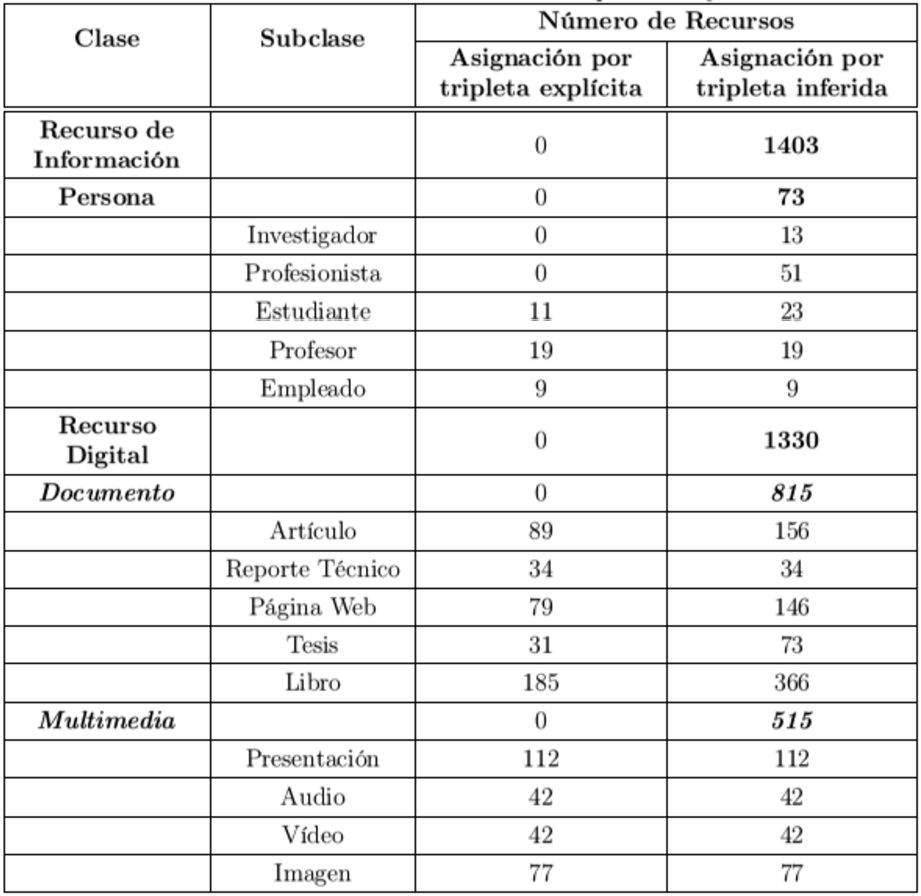
\includegraphics[scale=0.45]{NoRec} 
	\end{figure}
\end{frame}

\begin{frame}
	\frametitle{Diagrama de Venn asociado a los recursos digitales}
	%%%%%%%%%%%%%%%%%%%%%%%
	\begin{figure}
	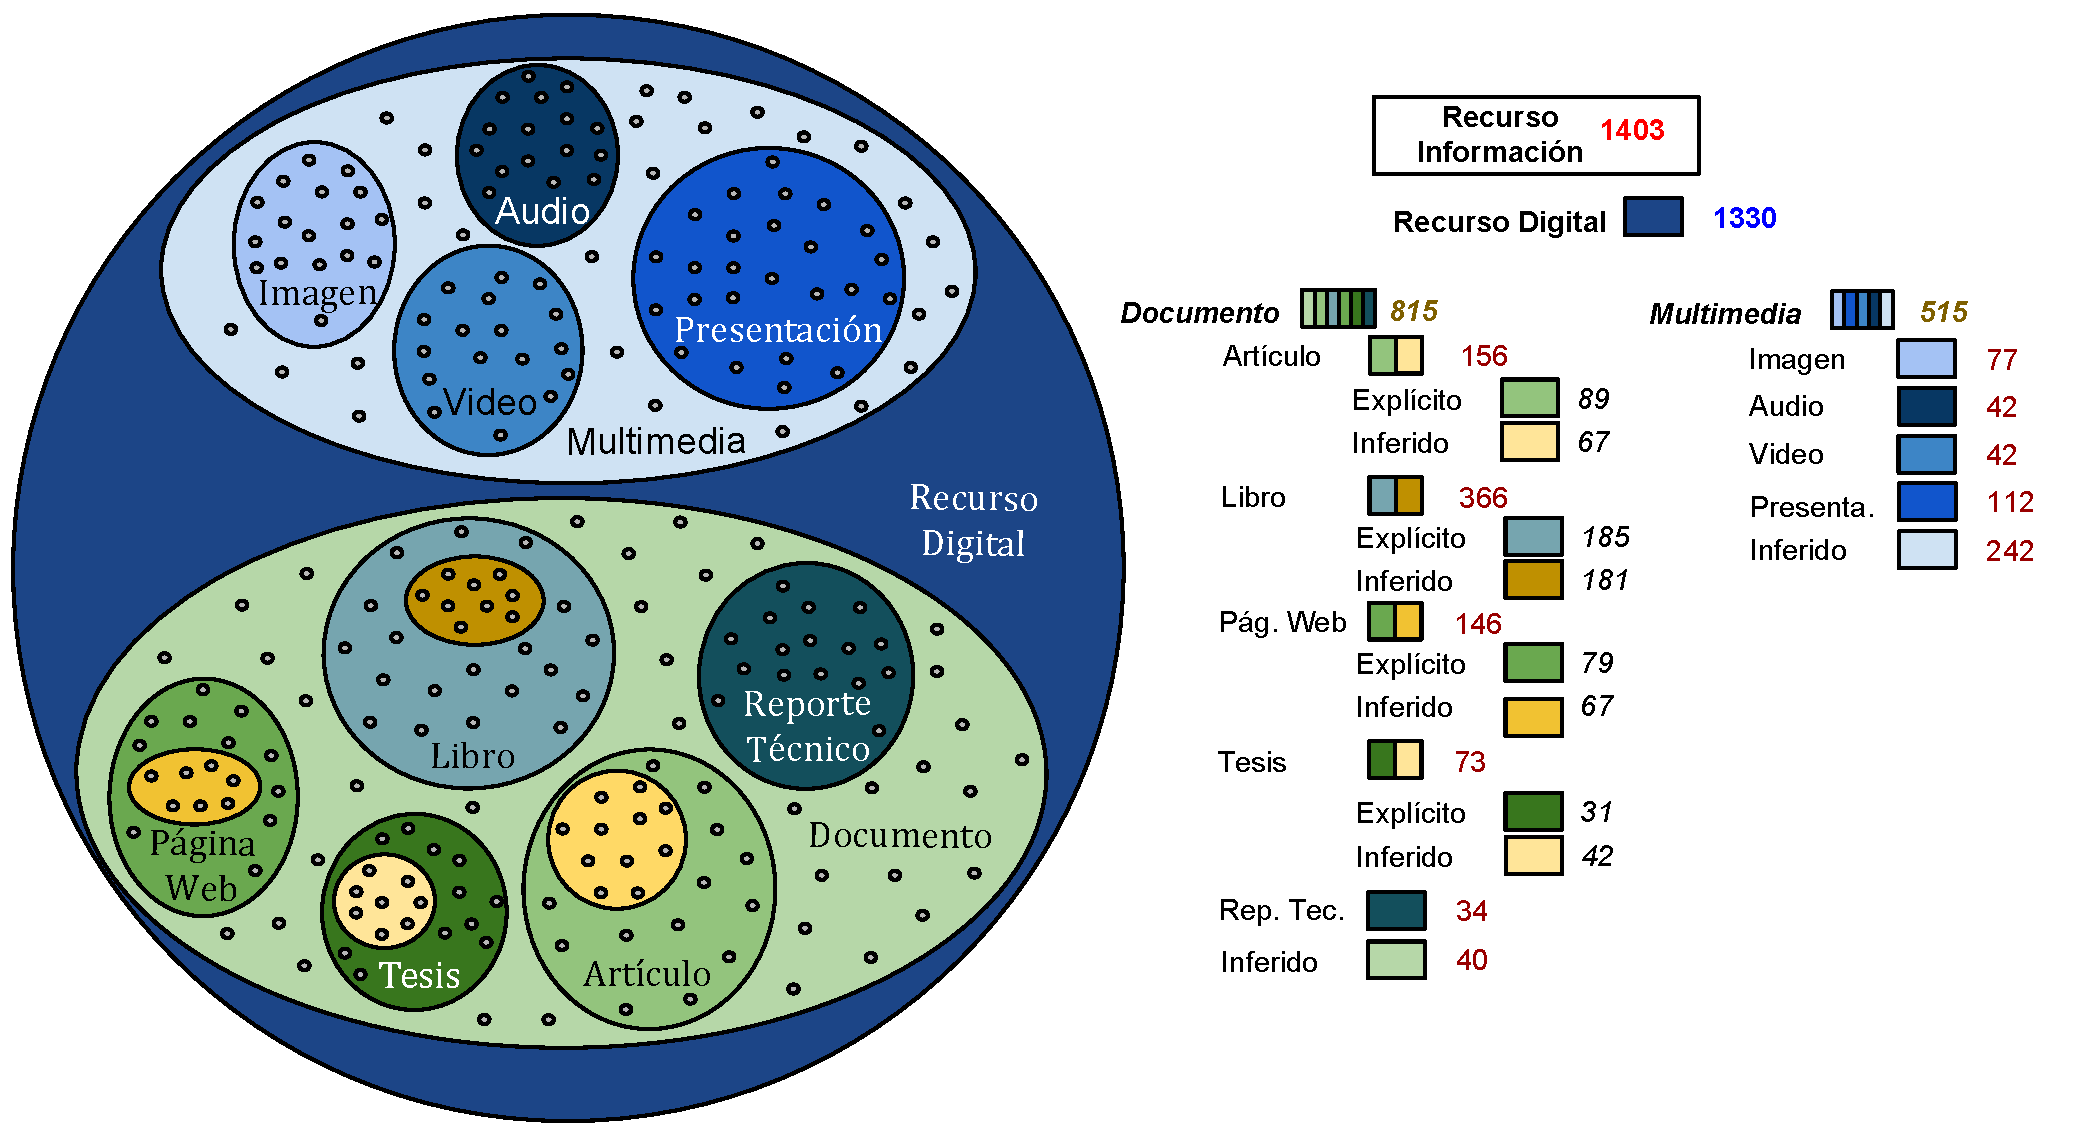
\includegraphics[scale=0.3]{ViewOnto} 
	\end{figure}
\end{frame}

\begin{frame}
	\frametitle{Preguntas en lenguaje natural}
	%%%%%%%%%%%%%%%%%%%%%%%
	\begin{figure}
	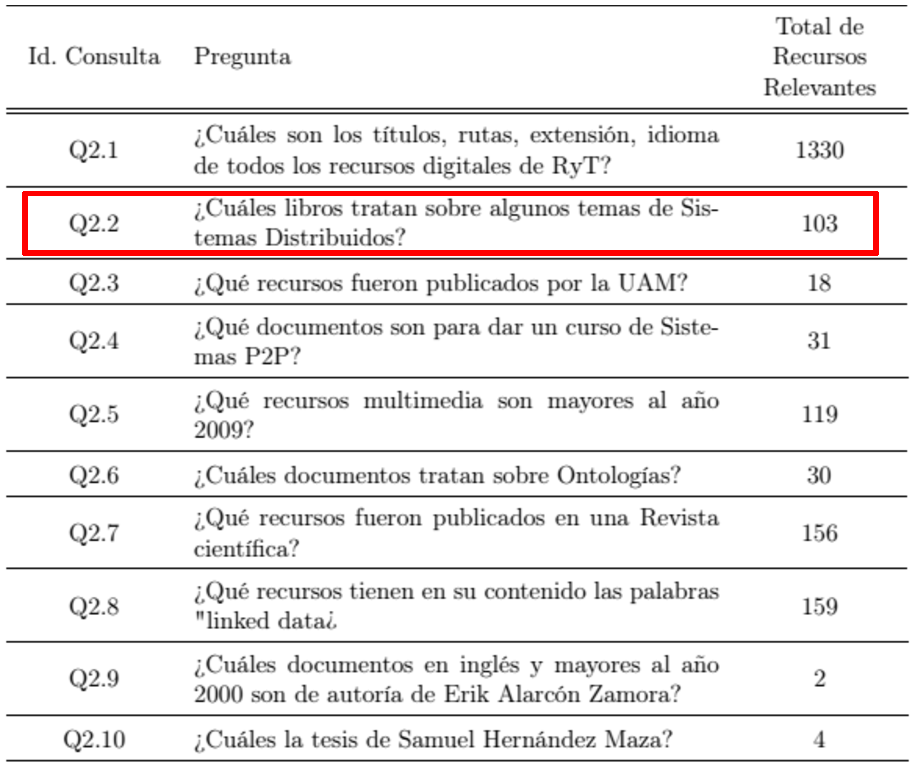
\includegraphics[scale=0.50]{Preguntas} 
	\end{figure}
\end{frame}
\section{Resultados}
\subsection{Resultados de la evaluaci�n}
\begin{frame}
	\begin{block}{}
	\justifying
	Q2.2.- �Cu�les libros tratan sobre algunos temas de Sistemas Distribuidos?
	\end{block}

	\frametitle{Calidad de los recursos recuperados}
	%%%%%%%%%%%%%%%%%%%%%%%
	\begin{figure}
	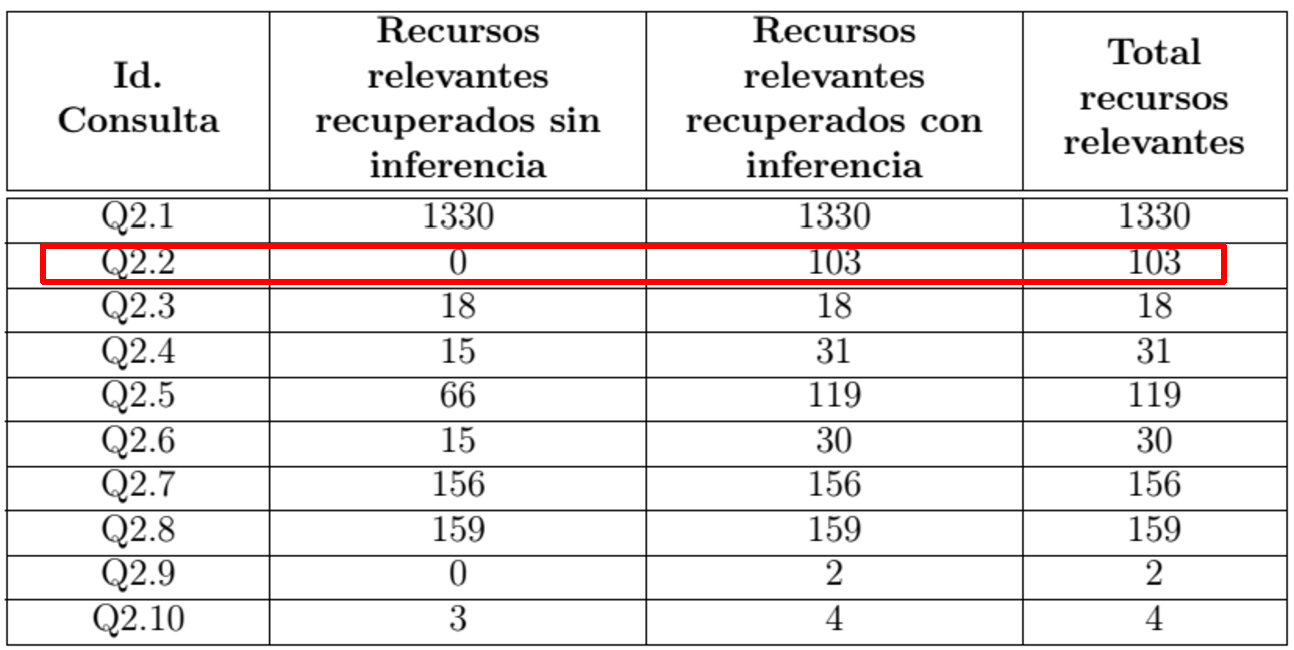
\includegraphics[scale=0.45]{Calidad} 
	\end{figure}
\end{frame}

\begin{frame}
	\frametitle{Exhaustividad y Precisi�n}
	\begin{block}{}
	\justifying
	Q2.2.- �Cu�les libros tratan sobre algunos temas de Sistemas Distribuidos?
	\end{block}

	\begin{figure}
	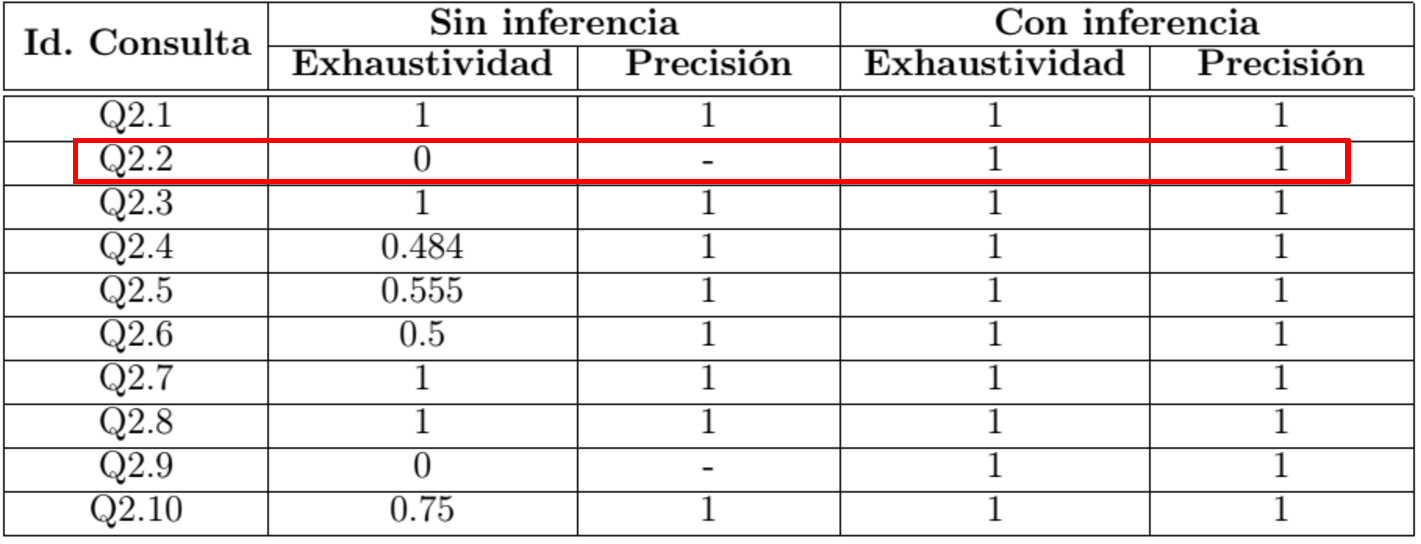
\includegraphics[scale=0.45]{ExahuPrecQ2} 
	\end{figure}
\end{frame}

\begin{frame}
	\begin{block}{}
	\justifying
	Q2.2.- �Cu�les libros tratan sobre algunos temas de Sistemas Distribuidos?
	\end{block}
	
	\frametitle{Tiempos de Procesamiento}
	%%%%%%%%%%%%%%%%%%%%%%%
	\begin{figure}
	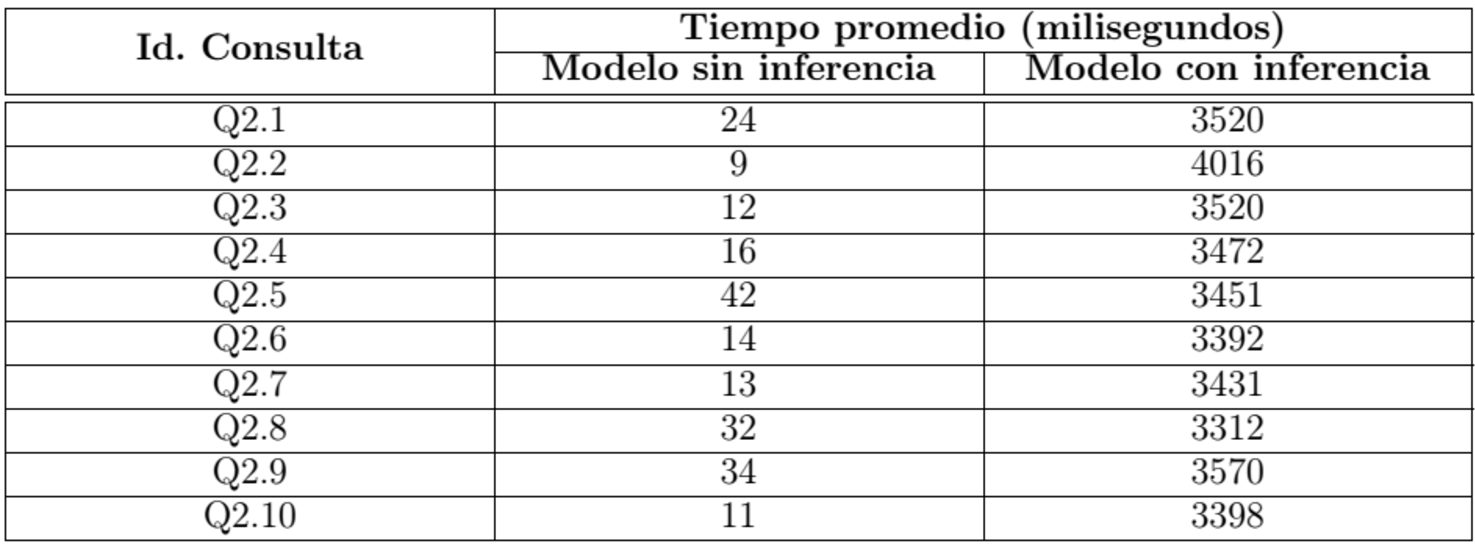
\includegraphics[scale=0.45]{Tiempos} 
	\end{figure}
\end{frame}

\subsection{Aportaciones}
\begin{frame}
	\frametitle{Aportaciones}
	\begin{figure}
	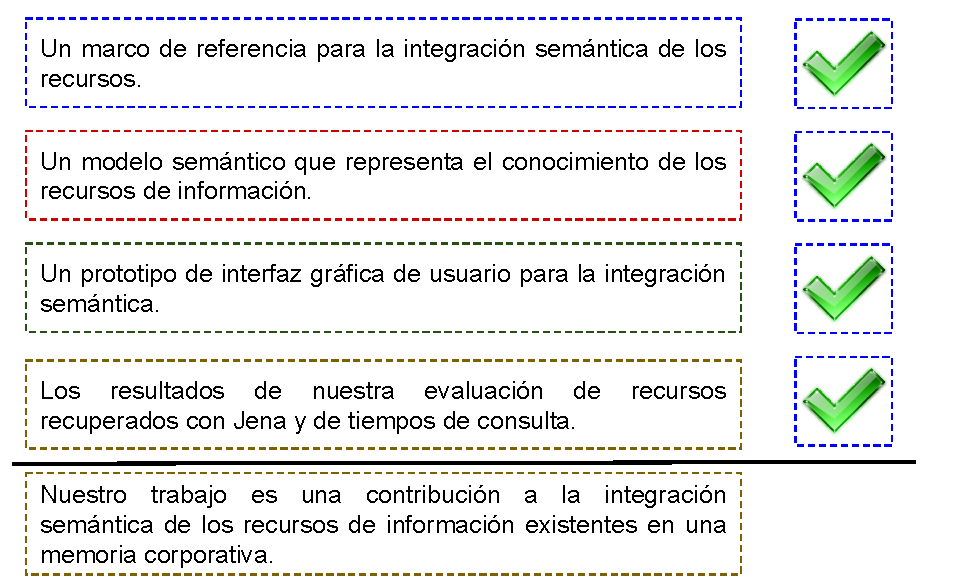
\includegraphics[scale=0.62]{ConclusionesObj} 
	\end{figure}
\end{frame}
\chapter{Conclusiones y Recomendaciones}
\label{cap:concl}
Con base en lo realizado y descrito en este documento, nosotros concluimos lo siguiente:

\begin{itemize}
\item Los objetivos particulares se alcanzaron:
	\begin{itemize}
	\item Desarrollamos un \textit{marco de referencia} para la \textit{integraci�n sem�ntica} de los \textit{recursos de informaci�n} existentes en una \textit{memoria corporativa}.
	\item Implementamos un \textit{modelo sem�ntico} que representa el conocimiento expl�cito e impl�cito de los \textit{recursos de informaci�n}.
	\item Implementamos un prototipo de interfaz gr�fica de usuario que permite a los usuarios una interacci�n amigable para la integraci�n sem�ntica de los recursos de informaci�n.
	\item Evaluamos los resultados devueltos y tiempos de procesamiento en la integraci�n sem�ntica para el dominio de redes y telecomunicaciones.
	\end{itemize}
\item Con respecto a nuestro objetivo principal, decimos que al alcanzar nuestros objetivos particulares, nosotros contribuimos a la \textit{integraci�n sem�ntica} de los \textit{recursos de informaci�n} existentes en una memoria corporativa.
\item La hip�tesis \textbf{El uso de las \textit{tecnolog�as sem�nticas} es adecuado para lograr la \textit{integraci�n sem�ntica} de \textit{recursos de informaci�n} en una \textit{memoria corporativa}}, se acepta porque las tecnolog�as sem�nticas son herramientas, est�ndares, metodolog�as y aplicaciones que permiten:
	\begin{itemize}
	\item Representar el conocimiento expl�cito (caracter�sticas y/o relaciones) de los \textit{recursos de informaci�n} en un modelo sem�ntico; solucionando las dificultades de heterogeneidad en formato, contenido y estructura.
	\item Enriquecer el conocimiento, mediante la introducci�n de \textit{reglas de inferencia} (Ver Secci�n \ref{sec:reginf} y \ref{sec:enrKrec}) en el modelo sem�ntico, para representar el conocimiento impl�cito en los recursos y el dominio de aplicaci�n (Redes y Telecomunicaciones).
	\item Extender o modificar un modelo sem�ntico, gracias a que el conocimiento expl�cito e impl�cito est�n escritos en un lenguaje est�ndar (Ver Secciones \ref{sec:rdf} y \ref{sec:reginf}). De esta manera, los modelos sem�nticos pueden adaptarse al conocimiento cambiante o explosivo de la memoria corporativa.
	\item Compartir un modelo sem�ntico, gracias a que �ste est� escrito en un lenguaje est�ndar y puede utilizarse en cualquier plataforma (Linux, Mac y Windows). De esta manera, mediante el uso de aplicaciones gen�ricas se puede visualizar o modificar la informaci�n en el modelo.
	\item Buscar y recuperar informaci�n en un modelo sem�ntico, mediante el uso de un lenguaje est�ndar (Ver Secci�n \ref{sec:lsparql}). As� como, el uso de un proceso para hacer expl�cito el conocimiento impl�cito de un modelo sem�ntico, con la finalidad de mejorar los resultados de la b�squeda en el modelo (Ver Secci�n \ref{sec:result}).
	\end{itemize}
\item Las aportaciones de nuestra investigaci�n son:
	\begin{itemize}
	\item Un \textit{marco de referencia} para lograr la integraci�n sem�ntica de recursos de informaci�n.
	\item Un modelo sem�ntico (ontolog�a) que representa el conocimiento de una memoria corporativa (Redes y Telecomunicaciones).
	\item Un prototipo para la b�squeda y consulta de informaci�n.
	\item Los resultados de nuestra evaluaci�n experimental.
	\item Un par de scripts para la generaci�n autom�tica y controlada de descripciones RDF, para poblar la base de conocimiento.
	\end{itemize}
\end{itemize}

%%%Qu� hicimos
En este documento presentamos un estudio y aplicaci�n sobre el uso de las \textit{tecnolog�as sem�nticas} (TS) para realizar la \textit{integraci�n sem�ntica} de los \textit{recursos de informaci�n} en una \textit{memoria corporativa}. Por \textit{integraci�n sem�ntica} debe entenderse la \textit{b�squeda y recuperaci�n} significativa de informaci�n existente en los \textit{recursos de informaci�n}. Estos recursos son documentos basados en texto y archivos multimedia en diferentes formatos, con contenido variado y con distintas estructuras (estructurado, semi-estructurado, sin estructura), tambi�n otros recursos de informaci�n en este trabajo son las personas.

%%%Por qu� hicimos �sto
Este trabajo tiene dos finalidades. Por un lado, esta investigaci�n propone un modelo sem�ntico (ontolog�a) que representa el conocimiento de una memoria corporativa, correspondiente al dominio de aplicaci�n de Redes y Telecomunicaciones. Conocimiento residente en personas y recursos digitales. Por otro lado, hacer la \textit{b�squeda y recuperaci�n inteligente de informaci�n} para responder las preguntas de los usuarios de la memoria.

%%Nuestro prototipo realmente f�cilita la interacci�n entre usuarios y un modelo sem�ntico.
As� mismo, nuestro trabajo propone un \textit{marco de referencia} para lograr la \textit{integraci�n sem�ntica de recursos} en una \textit{memoria corporativa}. Esta propuesta comprende tres actividades. La primera actividad es construir un modelo para representar el \textit{conocimiento expl�cito} de los \textit{recursos de informaci�n} existentes en una memoria corporativa. La segunda actividad es introducir \textit{reglas de inferencia} para enriquecer al modelo con conocimiento impl�cito existente en la memoria corporativa. La tercera actividad es \textit{buscar y recuperar informaci�n} existente en la memoria corporativa mediante la interrogaci�n del modelo sem�ntico.

%%%Qu� hicimos en cada etapa con las tecnolog�as sem�nticas
%%%Ventajas del uso de las tecnolog�as sem�nticas

Nosotros decidimos explorar las \textit{tecnolog�as sem�nticas} para la integraci�n de \textit{recursos de informaci�n} dadas las ventajas siguientes:

\begin{itemize}
\item El \textit{est�ndar RDF} permite representar cualquier recurso, sea un ser vivo, un archivo digital, un pa�s, ciudad, un edificio, una organizaci�n o un concepto abstracto. De esta manera, se contribuye a la integraci�n de informaci�n de \textit{recursos de informaci�n} que son heterog�neos en formato, contenido y estructura.
\item El \textit{est�ndar RDF} establece que los recursos tengan un identificador �nico de recurso (URI), para identificar de manera �nica a un recurso. De esta forma, se solucionan problemas de homonimia con respecto a los nombres de los recursos.
\item La representaci�n del contenido (caracter�sticas) de los \textit{recursos de informaci�n} de una memoria corporativa no se limita a un peque�o n�mero de caracter�sticas sobre �stos; sino que pueden vincularse estos recursos con otros a trav�s de relaciones o caracter�sticas m�s espec�ficas.
\item La introducci�n de \textit{reglas de inferencia} en la ontolog�a para enriquecer el conocimiento representado a trav�s de ella, ya que un razonador a partir de estas reglas puede hacer expl�cito el conocimiento impl�cito.
\item Una \textit{ontolog�a} puede ser extendida con el fin de \textit{incorporar mayor conocimiento} o \textit{adaptarse a cambios en el conocimiento}. De esta manera, si nuevos recursos se describen, entonces �stos pueden incorporarse a la ontolog�a. Ahora bien, si cambia el conocimiento en algunas ramas de la ontolog�a, entonces �stas pueden ser sustituidas por otras.
\item Una \textit{ontolog�a} est� escrita en un lenguaje est�ndar (OWL o RDF(S)) y representan un vocabulario consensuado por los expertos. Por esta raz�n, �stas se pueden intercambiar y reutilizar entre personas y/o aplicaciones.
\item Una \textit{ontolog�a} puede representarse de varias formas: a trav�s de un grafo dirigido o \textit{tripletas} (sujeto predicado objeto), cualquiera de ellas permite comprender los recursos as� como las reglas de inferencia.
\item Una \textit{ontolog�a} fomenta el desarrollo de aplicaciones gen�ricas para aprovechar estos modelos. Ejemplos de estas aplicaciones son editores de ontolog�as, interfaces gr�ficas para describir sem�nticamente los recursos, navegadores sobre ontolog�as, por mencionar algunas. Estas herramientas gen�ricas posibilitan que personas expertas en el dominio sean las principales constructoras del grafo de conocimiento. De esta manera, la informaci�n en el grafo ser� confiable, ya que estas personas son las que tienen los conocimientos en el dominio.
\end{itemize}

%Otras ventajas de tener ontolog�as en un formato est�ndar, son:
%\begin{itemize}
%\item Realizar tareas de inferencia a partir de los vocabularios OWL y RDF(S).
%\item Liberar a las organizaciones del uso de formatos propietarios que tienen un costo econ�mico o de propiedad intelectual.
%\item Construir r�pidamente modelos de conocimiento a partir de ontolog�as b�sicas.
%\item Mezclar ontolog�as y construir modelos de conocimiento complejos.
%\end{itemize}

%%%Ventajas de nuestra propuesta en relaci�n a otros trabajos
%Este \textit{marco de trabajo} emplea a los \textit{casos de uso} para guiar el proceso de \textit{integraci�n sem�ntica}. El primer \textit{caso de uso} es la \textit{cartograf�a de competencias} que consiste en encontrar personas con base a sus habilidades y capacidades profesionales, as� como conocimientos en los temas del dominio de la memoria. El segundo caso es la \textit{b�squeda de recursos digitales} que consiste en encontrar los \textit{documentos y recursos multimedia} a partir de la informaci�n sobre �stos (metadatos), en particular, encontrar recursos por los temas del dominio en la memoria.

%Estos dos \textit{casos de uso} son independientes entre s�, por ello, este marco propone la construcci�n de dos modelos u ontolog�as. La primera ontolog�a tiene el conocimiento expl�cito e impl�cito acerca de los \textit{recursos persona}. De la misma manera, la segunda ontolog�a tiene el conocimiento de los \textit{recursos digitales}. Un aspecto importante en ambos \textit{casos de uso} es vincular a cualquier recurso con los temas del dominio de la memoria corporativa. Por esta raz�n, se construye una tercera ontolog�a con los temas del dominio, donde estos temas est� jerarquizados.

%%%Para qui�n lo hicimos y con que prop�stio
%Esta propuesta se implemento para la memoria corporativa del �rea de Redes y Telecomunicaciones que pertenece al departamento de Ingenier�a El�ctrica de la Universidad Aut�noma Metropolitana. Por ello, la primera ontolog�a tiene informaci�n sobre profesores, alumnos y colegas que est�n vinculados con esta �rea. La segunda ontolog�a tienen informaci�n sobre los recursos digitales que representan trabajos, investigaciones, notas de curso, proyectos, tesis de las personas del �rea RyT. La tercera ontolog�a tiene los temas del �rea de RyT que est�n jerarquizados en cuatro ramas: \textit{sistemas distribuidos}, redes y servicios de telecomunicaciones, sistemas de comunicaci�n digital y web sem�ntica.

%%% que ventajas tiene nuestro prototipo en relacion con otros que se han examinado
La tarea de b�squeda y recuperaci�n de informaci�n son actividades que no cualquier usuario puede llevar a cabo, porque es necesario que tenga conocimientos sobre las tecnolog�as sem�nticas, as� como estar familiarizado en el dominio de conocimiento. Por esta raz�n, nosotros proponemos en esta investigaci�n un modelo (ontolog�a de Redes y Telecomunicaciones) y un prototipo (aplicaci�n) para permitir la interacci�n de cualquier usuario con el modelo, con fines de b�squeda y recuperaci�n de informaci�n en la memoria corporativa de trabajo (Redes y Telecomunicaciones).

La interfaz de nuestro prototipo est� orientada al usuario, es decir, un ambiente visual que permite una manera agradable para consultar la informaci�n de los recursos en nuestra ontolog�a. Esta caracter�stica es importante, porque en los trabajos de nuestro \textit{estado del arte} (Ver Secci�n \ref{sec:eoaisr}), ninguna aplicaci�n est� orientada al usuario.

Este prototipo establece las siguientes funcionalidades: 1) permitir a los usuarios, navegar a trav�s de la informaci�n b�sica en los \textit{recursos de informaci�n}, 2) permitir a los usuarios, estructurar sus preguntas y hacer b�squedas espec�ficas de los recursos, 3) publicar los resultados de la b�squeda y navegaci�n en un formato visual agradable, 4) transformar la preguntas a consultas SPARQL, 5) cargar las ontolog�as en memoria, 6) emplear un razonador para hacer expl�cito el conocimiento impl�cito de nuestro modelo sem�ntico.

%%%Conclusiones sobre la experimentaci�n
Nosotros llevamos a cabo una evaluaci�n experimental. Los objetivos de esta evaluaci�n son: 1) \textit{evaluar la calidad de los resultados de Jena para los modelos con y sin inferencia}, as� como 2) \textit{medir los tiempos promedio de procesamiento de Jena para las consultas de nuestra primera actividad}. En la medici�n de tiempos, quer�amos ver el rendimiento de Jena con la cantidad de datos que esperamos manejar. Mientras, en la evaluaci�n de resultados, quer�amos ver si los resultados devueltos por Jena, son los que responden nuestras preguntas.

Los resultados en nuestra experimentaci�n indican lo siguiente. El \textit{tiempo de consulta} es mayor en un \textit{modelo con inferencia} en comparaci�n con un \textit{modelo sin inferencia}. Sin embargo, los resultados de las b�squedas en un modelo sin inferencia son variados. En algunos casos, todos los \textit{resultados} que se sabe responden la consulta, son recuperados cuando la consulta es sobre el conocimiento expl�cito. En otros casos, recursos que responden la consulta, son descartados dado que estos recursos carecen de su descripci�n (tripleta) en la base de conocimiento. En cambio, los resultados de b�squedas sobre un \textit{modelo con inferencia} son buenos, porque estas consultas recuperan todos los recursos que de antemano sabemos que responden a las consultas; a pesar de no tener una descripci�n (tripleta) en la base de conocimiento.

Respecto a los tiempos, se tiene lo siguiente: el proceso de consulta sin inferencia arroja tiempos menores a un segundo, mientras los tiempos en la consulta con inferencia son de al rededor de dos o tres segundos. Aunque, los tiempos con inferencia son mayores en comparaci�n de los tiempos sin inferencia, a�n estos tiempos con inferencia son aceptables para la b�squeda de informaci�n basada en ontolog�as.

%%%Conclusi�n final, es factible o no es factible el uso de las TS y describir porqu�

%En este trabajo presentamos nuestro \textit{marco de trabajo}, un prototipo para la consulta de informaci�n, los resultados en nuestra evaluaci�n experimental, as� como las ventajas de las tecnolog�as sem�nticas, y con base en �stos, nosotros hacemos esta conclusi�n. 

%%% Trabajos futuros
\section{Recomendaciones}
En esta investigaci�n, nosotros identificamos varias actividades que consideramos como trabajos futuros:

\begin{itemize}
\item \textbf{A corto plazo:}
	\begin{itemize}
	\item Introducir m�s \textit{casos de uso}, por ejemplo, la administraci�n del inventario en los distintos laboratorios que componen el departamento de ingenier�a el�ctrica de la UAM.
	\item Actualizar los \textit{recursos de informaci�n} y las descripciones de �stos, para tener una buena representaci�n de la memoria corporativa del �rea de Redes y Telecomunicaciones.
	\item Evaluar la introducci�n de \textit{reglas de inferencia} m�s complejas en la ontolog�a, mediante el an�lisis de las reglas existentes y el uso de reglas del lenguaje \textit{Semantic Web Rule Language} \cite{SWRL} (SWRL), por ejemplo, si X es pariente de Z y Y tiene como hermano a K, entonces X es sobrino de K.
	\item Mejorar el prototipo de integraci�n sem�ntica de recursos:
		\begin{itemize}
		\item Agregar un cuadro para hacer b�squedas por palabras clave, mediante Lucene Index \cite{Lucene}.
		\item Optimizar los \textit{tiempos de procesamiento} en la b�squeda, por ejemplo, generando nuevas tripletas (materializando) desde el inicio las tripletas y almacen�ndolas en un nuevo modelo.
		\item Mejorar la manera en que se muestra la informaci�n de los recursos respuesta para una pregunta dada, mediante el uso del plug-in DataTables \cite{DataTables}.
		\item Mejorar la seguridad en la interfaz Web: autenticaci�n, autorizaci�n y administraci�n de sesiones, mediante el uso del marco de seguridad Apache Shiro \cite{Shiro}.
	\end{itemize}
	\end{itemize}
\item \textbf{A mediano plazo:}
	\begin{itemize}
	\item Automatizar la caracterizaci�n de los \textit{recursos de informaci�n}, mediante el uso de miner�a de texto.
	\item Mejorar la interfaz gr�fica de usuario del prototipo para que �ste pueda describir los \textit{recursos de informaci�n}. El objetivo es que los usuarios empleen esta aplicaci�n como una del estilo ``red social''. Algunas funcionalidades de esta interfaz son:
		\begin{itemize}
			\item Describir un nuevo \textit{recurso de informaci�n}.
			\begin{itemize}
				\item Asignar un identificador �nico de recurso al nuevo recurso de informaci�n.
				\item Construir un conjunto de tripletas RDF, asociadas al nuevo recurso de informaci�n.
				\item Guardar las tripletas en un archivo o agregar inmediatamente �stas al modelo sem�ntico.
			\end{itemize}
			\item Actualizar la informaci�n de un \textit{recurso de informaci�n}.
			\begin{itemize}
				\item Corregir la informaci�n en el modelo.
				\item Guardar el nuevo modelo.
			\end{itemize}
			\item Eliminar las descripciones de un \textit{recurso de informaci�n}.
			\begin{itemize}
				\item Ver la informaci�n del recurso a eliminar.
				\item Eliminar las tripletas en el modelo, donde el recurso es el sujeto.
				\item Guardar el nuevo modelo.
			\end{itemize}
		\end{itemize}
	\item Utilizar otro triplestore, por ejemplo Stardog \cite{Clark} o Sesame \cite{Aduna}, y hacer una evaluaci�n del mismo.
		\begin{itemize}
		\item Cargar, inferir y consultar nuestras ontolog�as con el \textit{triplestore electo}.
		\item Hacer nuestra evaluaci�n experimental con este triplestore.
		\item Comparar el desempe�o y resultados de experimentaci�n del \textit{triplestore electo} contra \textit{Jena}.
		\end{itemize}
	\item Dar mantenimiento a la ontolog�a del vocabulario de Redes y Telecomunicaciones.
		\begin{itemize}
		\item Introducir nuevos conceptos, como radios cognitivos, computaci�n en la nube, computaci�n m�vil, por mencionar algunos.
		\item Introducir tripletas para traducir los conceptos de nuestra ontolog�a a otros idiomas, por ejemplo, semantic web, web sem�ntica, web sem\^{a}ntica, semantisch web, anlamsal web, web semantikoa. De esta manera, en una b�squeda se pueden enriquecer los resultados, recuperando recursos que est�n en otros idiomas.
		\end{itemize}
	\end{itemize}
\end{itemize}

%%%%%%%%%%----------->Hay que expandir el cap�tulo con m�s ventajas de las TS

%Este cap�tulo est� bien escrito en general; pero es demasiado concreto. Hay que expandir las ventajas de la utilizaci�n de las tecnolog�as sem�nticas para vender la tesis mejor :).
\title{Integraci�n sem�ntica de \\ los recursos de informaci�n en \\ una memoria corporativa}
\author{Erik Alarc�n Zamora}
\date{Enero 2014. M�xico, D.F.}

\begin{frame}
\titlepage
\centering
Asesores:\\ Dra. Reyna Carolina Medina Ram�rez \\Dr. H�ctor P�rez Urbina
\\
\end{frame}
\input{anexos}

%\section{Referencias}
%\begin{frame}[allowframebreaks]
%\frametitle{Referencias}
%\begin{scriptsize} \bibliographystyle{apalike}
%\justifying \bibliography{bibliografia}\end{scriptsize}
%\end{frame}

\end{document}
